\documentclass[11pt,a4paper]{article}

% ---------------------------------------------------------------
% Packages
% ---------------------------------------------------------------
\usepackage[margin=1in]{geometry}
\usepackage{amsmath,amssymb,amsthm}
\usepackage{graphicx}
\usepackage{booktabs}
\usepackage{array}
\usepackage{float}
\usepackage[labelfont=bf,font=small]{caption}
\usepackage{algorithm}
\usepackage{algpseudocode}
\usepackage{enumitem}
\usepackage{tikz}
\usepackage[colorlinks=true,linkcolor=blue!50!black,citecolor=blue!50!black,urlcolor=blue!50!black]{hyperref}

\graphicspath{{./}{figures/}}

% ---------------------------------------------------------------
% Shortcuts
% ---------------------------------------------------------------
\newcommand{\dd}{\mathrm{d}}
\newcommand{\R}{\mathbb{R}}
\newcommand{\Dt}{\Delta t}
\newcommand{\bfy}{\mathbf{y}}
\newcommand{\bff}{\mathbf{f}}
\newtheorem{remark}{Remark}
\newtheorem{theorem}{Theorem}[section]

\setlength{\parskip}{4pt}
\setlength{\parindent}{0pt}

% ---------------------------------------------------------------
\begin{document}

\begin{titlepage}
\centering
\vspace*{2.5cm}
{\LARGE\bfseries Runge--Kutta Methods and Their Applications\par}
\vspace{0.5cm}
{\large From ODEs to PDEs by the Method of Lines:\\
the Heat Equation, the Lorenz System and the Lid-Driven Cavity\par}
\vspace{2cm}
{\Large Tanish Bansal\par}
{\large Roll No.\ 231075\par}
\vspace{0.8cm}
Undergraduate Project (UGP)\\
Indian Institute of Technology Kanpur\par
\vspace{0.8cm}
Supervisor: Prof.\ Saktipada Ghorai\par
\vspace{1.5cm}
October 30, 2026\par
\vfill
\begin{abstract}
\noindent
This report studies the classical fourth-order Runge--Kutta method (RK4) and three problems on which it
can be tested. After setting up the Butcher tableau and the rooted-tree theory of order (following
Chapter~3 of Butcher's book), we verify that RK4 satisfies the eight order conditions up to order four
and fails all nine conditions of order five, and we recall the linear stability function. The method is then applied to (i) the one-dimensional heat equation, converted into a
system of ordinary differential equations (ODEs) by the method of lines; (ii) the Lorenz system, a
nonlinear chaotic ODE; and (iii) the two-dimensional lid-driven cavity problem in the
streamfunction--vorticity form, again reduced to an ODE system in space. Every figure in the report is
produced by one Python script. On the heat equation we measure a temporal order of $4.08$ for RK4
and $1.00$ for the Euler method, a spatial order of $2.00$, and we observe that a mode driven $5\%$ past
the stability limit $|z|=2.7853$ grows by a factor $1.231$ per step while one $5\%$ inside decays by
$0.810$ per step. For the Lorenz system we reproduce the strange attractor at $\rho=28$, a decay to a
steady convection state at $\rho=10$ and a periodic orbit at $\rho=100$. For the cavity at Reynolds
number $100$ the RK4 time-marching reaches a steady state at $t\approx 31$, and the centre-line
velocity profiles agree with the benchmark data of Ghia, Ghia and Shin to within $0.006$.
\end{abstract}
\end{titlepage}

\tableofcontents
\newpage

% ===============================================================
\section{Introduction}
% ===============================================================

Most mathematical models of physical processes eventually reduce to the task of advancing a system of
ordinary differential equations in time. Runge--Kutta (RK) methods are among the most widely used tools
for this job: they are one-step methods, they need no special starting procedure, and the classical
four-stage member of the family, RK4, achieves fourth-order accuracy with only four evaluations of the
right-hand side per step.

The aim of this project was to understand RK methods and then to see where they can be used. The work
followed the reading material supplied by the supervisor~\cite{ghorai} together with standard
references~\cite{butcher2008,hairer1993}, and was organised in three steps.

\begin{enumerate}[leftmargin=*]
\item \textbf{Theory of RK methods} (Section~\ref{sec:rk}), following Chapter~3 of Butcher's
book~\cite{butcher2008}: the general form of an RK method and its Butcher tableau; rooted trees,
elementary differentials and elementary weights; the order theorem and the verification that RK4 has order
exactly four; local and global truncation error; low-order explicit methods, simplifying assumptions and
order barriers; error estimation with embedded pairs; and the stability function that limits the time step.
\item \textbf{From PDE to ODE} (Section~\ref{sec:mol}): since RK methods solve ODEs, a partial
differential equation has first to be discretised in space. This is the \emph{method of lines}. It is
illustrated on the heat equation, for which the exact solution is known, so that the theory can be
checked quantitatively (Section~\ref{sec:heatexp}).
\item \textbf{Applications}: the Lorenz equations (Sections~\ref{sec:lorenz} and~\ref{sec:lorenzexp}), an
ODE problem that is nonlinear and chaotic, and the lid-driven cavity problem (Section~\ref{sec:cavity}),
a nonlinear PDE problem that combines the method of lines with an elliptic (Poisson) solve at every step.
\end{enumerate}

All numerical results were produced with a single Python/NumPy/SciPy script (\texttt{experiment.py}),
which writes the seven figures used below. Each figure is placed next to the experiment it belongs to.

\paragraph{Notation.} The ODE is written $\bfy'(t)=\bff(\bfy(t))$, $\bfy\in\R^M$; the time step is
$\Dt$ (also written $h$ in the general theory) and the space step is $h_s$ or $h$ where the context is
clear. The Euler method is called ``Euler'' throughout.

% ===============================================================
\section{Runge--Kutta Methods}\label{sec:rk}
% ===============================================================

\subsection{The initial value problem and the Euler method}

We consider the autonomous initial value problem (IVP)
\begin{equation}
\bfy'(t)=\bff(\bfy(t)),\qquad \bfy(t_0)=\bfy_0 .
\label{eq:ivp}
\end{equation}
Non-autonomous problems can be brought to this form by adding $t$ as an extra variable, so no
generality is lost. The simplest method is the Euler method, which follows the tangent line for one step,
\begin{equation}
\bfy_{n+1}=\bfy_n+\Dt\,\bff(\bfy_n).
\end{equation}
Taylor expansion shows that the local error is $\tfrac12\Dt^2\bfy''+O(\Dt^3)$, so the method is of
first order.

\subsection{General explicit and implicit RK methods}

An $s$-stage RK method uses $s$ intermediate \emph{stages} $Y_1,\dots,Y_s$ to build one step:
\begin{equation}
Y_i=\bfy_n+\Dt\sum_{j=1}^{s}a_{ij}\,\bff(Y_j),\qquad
\bfy_{n+1}=\bfy_n+\Dt\sum_{i=1}^{s}b_i\,\bff(Y_i),\qquad c_i=\sum_{j}a_{ij}.
\label{eq:rkgeneral}
\end{equation}
The coefficients are collected in the \emph{Butcher tableau}
\begin{equation}
\begin{array}{c|c}
\mathbf{c} & A\\ \hline
 & \mathbf{b}^{T}
\end{array}
=
\begin{array}{c|cccc}
c_1 & a_{11} & a_{12} & \cdots & a_{1s}\\
c_2 & a_{21} & a_{22} & \cdots & a_{2s}\\
\vdots & \vdots & \vdots & \ddots & \vdots\\
c_s & a_{s1} & a_{s2} & \cdots & a_{ss}\\ \hline
 & b_1 & b_2 & \cdots & b_s
\end{array}
\end{equation}
The structure of $A$ decides how the method is computed.
\begin{itemize}[leftmargin=*]
\item \textbf{Explicit} (ERK): $A$ is strictly lower triangular. The stages are computed one after the
other, with no equation solving. This is cheap per step.
\item \textbf{Implicit} (IRK): $A$ is a full matrix. All stages are coupled, and every step needs the
solution of $sM$ nonlinear equations, typically by Newton's method.
\item \textbf{Diagonally implicit} (DIRK): $A$ is lower triangular with a non-zero diagonal. The stages
are still computed one after the other, but each needs the solution of an $M$-dimensional nonlinear
system. If all diagonal entries are equal (SDIRK), a single LU factorisation of $I-\Dt\,a_{ii}J$ can be
reused for all stages.
\end{itemize}

\paragraph{Euler and RK4 as tableaux.} The Euler method is the one-stage method with $b_1=1$,
$a_{11}=0$. The classical RK4 method has the tableau
\begin{equation}
\begin{array}{c|cccc}
0 & 0 & & & \\
\tfrac12 & \tfrac12 & 0 & & \\
\tfrac12 & 0 & \tfrac12 & 0 & \\
1 & 0 & 0 & 1 & 0\\ \hline
 & \tfrac16 & \tfrac13 & \tfrac13 & \tfrac16
\end{array}
\end{equation}
which written out is
\begin{align}
k_1&=\bff(\bfy_n), & k_2&=\bff\!\left(\bfy_n+\tfrac{\Dt}{2}k_1\right),\notag\\
k_3&=\bff\!\left(\bfy_n+\tfrac{\Dt}{2}k_2\right), & k_4&=\bff(\bfy_n+\Dt\,k_3),\notag\\
\bfy_{n+1}&=\bfy_n+\tfrac{\Dt}{6}\,(k_1+2k_2+2k_3+k_4).
\label{eq:rk4}
\end{align}
The weights $\tfrac16,\tfrac13,\tfrac13,\tfrac16$ are those of Simpson's rule. The cost per step is four
evaluations of $\bff$ for RK4 against one for Euler.

\begin{algorithm}[H]
\caption{One step of classical RK4 for $\bfy'=\bff(\bfy)$}\label{alg:rk4}
\begin{algorithmic}[1]
\Require current state $\bfy_n$, step size $\Dt$, function $\bff$
\State $k_1\gets \bff(\bfy_n)$
\State $k_2\gets \bff(\bfy_n+\tfrac12\Dt\,k_1)$
\State $k_3\gets \bff(\bfy_n+\tfrac12\Dt\,k_2)$
\State $k_4\gets \bff(\bfy_n+\Dt\,k_3)$
\State \Return $\bfy_{n+1}\gets \bfy_n+\tfrac{\Dt}{6}\,(k_1+2k_2+2k_3+k_4)$
\end{algorithmic}
\end{algorithm}

\subsection{Rooted trees and functions on trees}\label{sec:trees}

The accuracy analysis of RK methods rests on a combinatorial object, the \emph{rooted tree}, which we
introduce following Butcher~\cite[Sect.~30]{butcher2008}. A rooted tree is a finite set of
\emph{vertices} together with a set of \emph{edges}, each edge being an ordered pair $[x,y]$ ($x$ is the
\emph{parent} and $y$ the \emph{child}). Exactly one vertex, the \emph{root}, has no parent; every other
vertex has exactly one parent; and the graph is connected. A vertex without children is a \emph{leaf}.
Two trees that differ only in the names of their vertices are regarded as the same \emph{abstract} tree.
We write $\vartheta$ for a tree (the letter $t$ is kept for time) and draw the root at the bottom.

\paragraph{Notation.} The tree with one vertex is $\tau$. If removing the root of $\vartheta$ leaves the
subtrees $\vartheta_1,\dots,\vartheta_m$, we write $\vartheta=[\vartheta_1\,\vartheta_2\cdots\vartheta_m]$,
and repeated subtrees are written as powers; for example $[\tau\,\tau\,[\tau]]=[\tau^2[\tau]]$.
All trees with up to four vertices are drawn in Figure~\ref{fig:trees}.

\begin{figure}[H]
\centering
\begin{minipage}[b]{0.115\textwidth}\centering
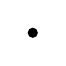
\begin{tikzpicture}[scale=0.55,every node/.style={circle,fill,inner sep=1.3pt}]
\node (a) at (0,0) {};
\end{tikzpicture}\\[2pt]\small $\tau$
\end{minipage}\hfill
\begin{minipage}[b]{0.115\textwidth}\centering
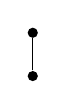
\begin{tikzpicture}[scale=0.55,every node/.style={circle,fill,inner sep=1.3pt}]
\node (a) at (0,0) {}; \node (b) at (0,1) {}; \draw (a)--(b);
\end{tikzpicture}\\[2pt]\small $[\tau]$
\end{minipage}\hfill
\begin{minipage}[b]{0.115\textwidth}\centering
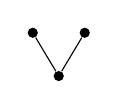
\begin{tikzpicture}[scale=0.55,every node/.style={circle,fill,inner sep=1.3pt}]
\node (a) at (0,0) {}; \node (b) at (-0.6,1) {}; \node (c) at (0.6,1) {};
\draw (a)--(b); \draw (a)--(c);
\end{tikzpicture}\\[2pt]\small $[\tau^2]$
\end{minipage}\hfill
\begin{minipage}[b]{0.115\textwidth}\centering
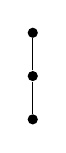
\begin{tikzpicture}[scale=0.55,every node/.style={circle,fill,inner sep=1.3pt}]
\node (a) at (0,0) {}; \node (b) at (0,1) {}; \node (c) at (0,2) {};
\draw (a)--(b)--(c);
\end{tikzpicture}\\[2pt]\small $[[\tau]]$
\end{minipage}\hfill
\begin{minipage}[b]{0.115\textwidth}\centering
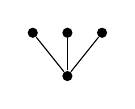
\begin{tikzpicture}[scale=0.55,every node/.style={circle,fill,inner sep=1.3pt}]
\node (a) at (0,0) {}; \node (b) at (-0.8,1) {}; \node (c) at (0,1) {}; \node (d) at (0.8,1) {};
\draw (a)--(b); \draw (a)--(c); \draw (a)--(d);
\end{tikzpicture}\\[2pt]\small $[\tau^3]$
\end{minipage}\hfill
\begin{minipage}[b]{0.115\textwidth}\centering
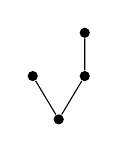
\begin{tikzpicture}[scale=0.55,every node/.style={circle,fill,inner sep=1.3pt}]
\node (a) at (0,0) {}; \node (b) at (-0.6,1) {}; \node (c) at (0.6,1) {}; \node (d) at (0.6,2) {};
\draw (a)--(b); \draw (a)--(c)--(d);
\end{tikzpicture}\\[2pt]\small $[\tau[\tau]]$
\end{minipage}\hfill
\begin{minipage}[b]{0.115\textwidth}\centering
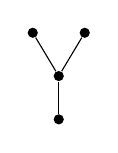
\begin{tikzpicture}[scale=0.55,every node/.style={circle,fill,inner sep=1.3pt}]
\node (a) at (0,0) {}; \node (b) at (0,1) {}; \node (c) at (-0.6,2) {}; \node (d) at (0.6,2) {};
\draw (a)--(b); \draw (b)--(c); \draw (b)--(d);
\end{tikzpicture}\\[2pt]\small $[[\tau^2]]$
\end{minipage}\hfill
\begin{minipage}[b]{0.115\textwidth}\centering
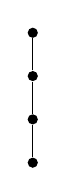
\begin{tikzpicture}[scale=0.55,every node/.style={circle,fill,inner sep=1.3pt}]
\node (a) at (0,0) {}; \node (b) at (0,1) {}; \node (c) at (0,2) {}; \node (d) at (0,3) {};
\draw (a)--(b)--(c)--(d);
\end{tikzpicture}\\[2pt]\small $[[[\tau]]]$
\end{minipage}
\caption{The eight rooted trees with at most four vertices, with the root at the bottom.}
\label{fig:trees}
\end{figure}

Three integers are attached to every tree.
\begin{itemize}[leftmargin=*]
\item The \emph{order} $r(\vartheta)$ is the number of vertices.
\item The \emph{symmetry} $\mathrm{sym}(\vartheta)$ is the order of the group of vertex relabellings that
leave the tree unchanged (denoted $\sigma(\vartheta)$ by Butcher; we avoid this letter because $\sigma$ is
a parameter of the Lorenz system).
\item The \emph{density} $\gamma(\vartheta)$ is the product, over all vertices, of the number of vertices
in the subtree that starts at that vertex.
\end{itemize}
If $\vartheta=[\vartheta_1^{m_1}\cdots\vartheta_k^{m_k}]$ with distinct $\vartheta_i$, then
\begin{equation}
r(\vartheta)=1+\sum_i m_i\,r(\vartheta_i),\qquad
\mathrm{sym}(\vartheta)=\prod_i m_i!\,\mathrm{sym}(\vartheta_i)^{m_i},\qquad
\gamma(\vartheta)=r(\vartheta)\prod_i\gamma(\vartheta_i)^{m_i},
\label{eq:treerec}
\end{equation}
with $r(\tau)=\mathrm{sym}(\tau)=\gamma(\tau)=1$ \cite[Thm.~301A]{butcher2008}. As an example, the tree with
nine vertices consisting of a root with two children, each of which has three leaves, has $r=9$,
$\mathrm{sym}=3!\,3!\,2!=72$ and $\gamma=1^6\cdot4\cdot4\cdot9=144$.

A fourth integer counts labellings. Let $\nu(\vartheta)$ be the number of ways of labelling the vertices with
$1,\dots,r(\vartheta)$ such that the labels increase along every edge, labellings that differ only by a
symmetry of the tree being counted once ($\nu$ is called $\alpha$ by Butcher; the letter $\alpha$ is the
diffusivity in the heat equation). Then \cite[Thm.~302A]{butcher2008}
\begin{equation}
\nu(\vartheta)=\frac{r(\vartheta)!}{\mathrm{sym}(\vartheta)\,\gamma(\vartheta)}.
\label{eq:nu}
\end{equation}
The number of trees of order $n=1,2,3,\dots,10$ is $1,1,2,4,9,20,48,115,286,719$, so the number of trees of
order at most $p$ is $1,2,4,8,17,37,\dots$ for $p=1,2,3,\dots$ \cite[Thm.~302B]{butcher2008}. This fast growth
is the reason why high-order methods are hard to construct: each tree gives one equation that the method
must satisfy.

\subsection{Elementary differentials and the Taylor series of the exact solution}\label{sec:elemdiff}

Differentiate $\bfy'=\bff(\bfy)$ repeatedly, using the chain rule and $\bfy'=\bff$:
\begin{align}
\bfy'&=\bff,\qquad \bfy''=\bff'\bff,\qquad \bfy'''=\bff''(\bff,\bff)+\bff'\bff'\bff,\notag\\
\bfy''''&=\bff'''(\bff,\bff,\bff)+3\,\bff''(\bff,\bff'\bff)+\bff'\bff''(\bff,\bff)+\bff'\bff'\bff'\bff .
\label{eq:derivs}
\end{align}
Here $\bff'$ is the Jacobian matrix and $\bff'',\bff'''$ are the bilinear and trilinear maps of the second
and third derivatives. Every term is a nested expression in $\bff$ and its derivatives, and each such
expression corresponds to a rooted tree: a vertex with $m$ children stands for the $m$-th derivative
$\bff^{(m)}$ applied to the expressions of its children, and a leaf stands for $\bff$ itself. This defines the
\emph{elementary differential} of a tree \cite[Sect.~310]{butcher2008}:
\begin{equation}
\mathbf F(\tau)=\bff,\qquad
\mathbf F([\vartheta_1\cdots\vartheta_m])=\bff^{(m)}\bigl(\mathbf F(\vartheta_1),\dots,\mathbf F(\vartheta_m)\bigr).
\end{equation}
Differentiating an elementary differential once more adds one vertex to the tree in every possible way,
which is why the multiplicity of a tree in the $n$-th derivative is exactly $\nu(\vartheta)$:
\begin{equation}
\bfy^{(n)}=\sum_{r(\vartheta)=n}\nu(\vartheta)\,\mathbf F(\vartheta)\quad\text{\cite[Thm.~311C]{butcher2008}.}
\end{equation}
For instance $\nu([\tau[\tau]])=3$, matching the coefficient $3$ of $\bff''(\bff,\bff'\bff)$ in~\eqref{eq:derivs}.
Dividing by $n!$ and using~\eqref{eq:nu}, the Taylor series of the exact solution becomes
\begin{equation}
\bfy(t+\Dt)=\bfy+\sum_{\vartheta}\frac{\Dt^{\,r(\vartheta)}}{\mathrm{sym}(\vartheta)\,\gamma(\vartheta)}\,\mathbf F(\vartheta)(\bfy).
\label{eq:exacttaylor}
\end{equation}
Butcher obtains the same result by a second route, by expanding the Picard iterates of
$\bfy(t+\Dt\xi)=\bfy(t)+\Dt\int_0^\xi\bff(\bfy(t+\Dt\zeta))\,\dd\zeta$ \cite[Thm.~311D]{butcher2008}.
Table~\ref{tab:trees} lists the trees up to order four with their integers and elementary differentials.

\begin{table}[H]
\centering
\begin{tabular}{@{}clcccc@{}}
\toprule
$r$ & tree $\vartheta$ & $\mathrm{sym}$ & $\gamma$ & $\nu$ & $\mathbf F(\vartheta)$\\
\midrule
1 & $\tau$ & 1 & 1 & 1 & $\bff$\\
2 & $[\tau]$ & 1 & 2 & 1 & $\bff'\bff$\\
3 & $[\tau^2]$ & 2 & 3 & 1 & $\bff''(\bff,\bff)$\\
3 & $[[\tau]]$ & 1 & 6 & 1 & $\bff'\bff'\bff$\\
4 & $[\tau^3]$ & 6 & 4 & 1 & $\bff'''(\bff,\bff,\bff)$\\
4 & $[\tau[\tau]]$ & 1 & 8 & 3 & $\bff''(\bff,\bff'\bff)$\\
4 & $[[\tau^2]]$ & 2 & 12 & 1 & $\bff'\bff''(\bff,\bff)$\\
4 & $[[[\tau]]]$ & 1 & 24 & 1 & $\bff'\bff'\bff'\bff$\\
\bottomrule
\end{tabular}
\caption{Rooted trees up to order four with their symmetry, density, number of monotone labellings and
elementary differential.}
\label{tab:trees}
\end{table}

\subsection{Elementary weights and the order theorem}\label{sec:orderthm}

The same trees organise the numerical solution. For the stage values $Y_i$ of~\eqref{eq:rkgeneral}, Butcher
defines recursively the \emph{internal weights} $\Phi_i$, \emph{derivative weights} $(\Phi_iD)$ and the
\emph{elementary weights} $\Phi$ of a tree \cite[Def.~312A]{butcher2008}:
\begin{equation}
(\Phi_iD)(\tau)=1,\qquad
\Phi_i(\vartheta)=\sum_{j=1}^{s}a_{ij}\,(\Phi_jD)(\vartheta),\qquad
(\Phi_iD)([\vartheta_1\cdots\vartheta_k])=\prod_{l=1}^{k}\Phi_i(\vartheta_l),\qquad
\Phi(\vartheta)=\sum_{i=1}^{s}b_i\,(\Phi_iD)(\vartheta).
\end{equation}
An equivalent rule \cite[Lemma~312B]{butcher2008} is the following. Give every vertex of the tree its own
stage index running over $1,\dots,s$; the root contributes $b_i$; each edge from a vertex with index $j$ to
a child with index $k$ contributes $a_{jk}$; multiply everything and sum over all indices. A leaf with index
$l$ can be summed first using $\sum_la_{kl}=c_k$. For example $\Phi(\tau)=\sum b_i$, $\Phi([\tau])=\sum b_ic_i$ and
$\Phi([[\tau]])=\sum b_ia_{ij}c_j$.

\begin{theorem}[Butcher: expansion of one RK step]\label{thm:rkexp}
The result of one step of an RK method has the formal Taylor series
\begin{equation}
\bfy_1=\bfy_0+\sum_{\vartheta}\frac{\Dt^{\,r(\vartheta)}}{\mathrm{sym}(\vartheta)}\,\Phi(\vartheta)\,\mathbf F(\vartheta)(\bfy_0),
\end{equation}
which is~\eqref{eq:exacttaylor} with $1/\gamma(\vartheta)$ replaced by $\Phi(\vartheta)$ \cite[Thm.~313B]{butcher2008}.
\end{theorem}

Comparing the two series term by term gives the criterion for order. This comparison is legitimate
because the elementary differentials cannot cancel each other: Butcher constructs, for any finite set of trees,
an ODE system whose elementary differentials at the initial point are independent unit vectors
\cite[Thm.~314A]{butcher2008}, and conversely any prescribed values of the weights $\Phi(\vartheta)$ on a finite set of trees
can be realised by some RK method \cite[Thm.~317A]{butcher2008}. So the conditions below are independent of each
other and cannot be reduced further.

\begin{theorem}[Order theorem]\label{thm:order}
An RK method has order $p$ if and only if
\begin{equation}
\Phi(\vartheta)=\frac1{\gamma(\vartheta)}\qquad\text{for every tree }\vartheta\text{ with }r(\vartheta)\le p
\quad\text{\cite[Thm.~315A]{butcher2008}.}
\end{equation}
\end{theorem}

For $p\le4$ these are the eight conditions of Table~\ref{tab:orderconds}. For ODEs of the scalar,
non-autonomous form $y'=f(x,y)$ the conditions for orders up to four are the same, but from order five the
two conditions for $[\tau[[\tau]]]$ and $[[\tau[\tau]]]$ (values $\tfrac1{30}$ and $\tfrac1{40}$) collapse to the
single condition $\sum b_ic_ia_{ij}a_{jk}c_k+\sum b_ia_{ij}c_ja_{jk}c_k=\tfrac7{120}$; for methods that satisfy the
$D(1)$ condition of Section~\ref{sec:simplify} the scalar and vector conditions are equivalent
\cite[Sect.~316]{butcher2008}.

\begin{table}[H]
\centering
\begin{tabular}{@{}clccc@{}}
\toprule
order & tree $\vartheta$ & $\Phi(\vartheta)$ & required $1/\gamma$ & RK4 value\\
\midrule
1 & $\tau$ & $\sum_i b_i$ & $1$ & $1$\\
2 & $[\tau]$ & $\sum_i b_ic_i$ & $\tfrac12$ & $\tfrac12$\\
3 & $[\tau^2]$ & $\sum_i b_ic_i^2$ & $\tfrac13$ & $\tfrac13$\\
3 & $[[\tau]]$ & $\sum_{i,j} b_ia_{ij}c_j$ & $\tfrac16$ & $\tfrac16$\\
4 & $[\tau^3]$ & $\sum_i b_ic_i^3$ & $\tfrac14$ & $\tfrac14$\\
4 & $[\tau[\tau]]$ & $\sum_{i,j} b_ic_ia_{ij}c_j$ & $\tfrac18$ & $\tfrac18$\\
4 & $[[\tau^2]]$ & $\sum_{i,j} b_ia_{ij}c_j^2$ & $\tfrac1{12}$ & $\tfrac1{12}$\\
4 & $[[[\tau]]]$ & $\sum_{i,j,k} b_ia_{ij}a_{jk}c_k$ & $\tfrac1{24}$ & $\tfrac1{24}$\\
\bottomrule
\end{tabular}
\caption{Order conditions up to order four. The last column is verified for RK4 below.}
\label{tab:orderconds}
\end{table}

\paragraph{Euler.} Only $\sum b_i=1$ holds; since $c_1=0$, $\sum b_ic_i=0\ne\tfrac12$. The order is one, and the
leading local error is $-\tfrac12\Dt^2\bff'\bff$, the first neglected Taylor term.

\paragraph{RK4.} With $\mathbf c=(0,\tfrac12,\tfrac12,1)$, $a_{21}=a_{32}=\tfrac12$, $a_{43}=1$:
\begin{align*}
\sum b_i c_i&=\tfrac13\cdot\tfrac12+\tfrac13\cdot\tfrac12+\tfrac16\cdot1=\tfrac12, &
\sum b_i c_i^2&=\tfrac13\cdot\tfrac14+\tfrac13\cdot\tfrac14+\tfrac16=\tfrac13,\\
\sum b_i c_i^3&=\tfrac13\cdot\tfrac18+\tfrac13\cdot\tfrac18+\tfrac16=\tfrac14, &
\sum b_i a_{ij}c_j&=\tfrac13\cdot\tfrac12\cdot\tfrac12+\tfrac16\cdot1\cdot\tfrac12=\tfrac16,\\
\sum b_ic_ia_{ij}c_j&=\tfrac13\cdot\tfrac12\cdot\tfrac14+\tfrac16\cdot1\cdot\tfrac12=\tfrac18, &
\sum b_ia_{ij}c_j^2&=\tfrac13\cdot\tfrac12\cdot\tfrac14+\tfrac16\cdot1\cdot\tfrac14=\tfrac1{12},\\
\sum b_ia_{ij}a_{jk}c_k&=\tfrac16\cdot1\cdot\tfrac12\cdot\tfrac12=\tfrac1{24}. &&
\end{align*}
All eight conditions hold, so RK4 has order at least four.

\subsection{RK4 is of order exactly four: the error coefficients}\label{sec:rk4err}

If the conditions hold up to order $p$, the leading term of the local error comes from the trees of order
$p+1$ \cite[Sect.~318]{butcher2008}:
\begin{equation}
\bfy_1-\bfy(t_0+\Dt)=\Dt^{\,p+1}\sum_{r(\vartheta)=p+1}\frac{1}{\mathrm{sym}(\vartheta)}
\Bigl(\Phi(\vartheta)-\frac1{\gamma(\vartheta)}\Bigr)\mathbf F(\vartheta)(\bfy_0)+O(\Dt^{p+2}).
\label{eq:lte}
\end{equation}
The elementary weights of RK4 for the nine trees of order five were computed with the recursive definition
above (using exact rational arithmetic) and are listed in Table~\ref{tab:order5}.

\begin{table}[H]
\centering
\begin{tabular}{@{}lcccc@{}}
\toprule
tree $\vartheta$ & $\gamma$ & $\Phi(\vartheta)$ & $\Phi-\tfrac1\gamma$ & $\gamma\Phi-1$\\
\midrule
$[\tau^4]$ & 5 & $\tfrac5{24}$ & $\tfrac1{120}$ & $\tfrac1{24}$\\
$[\tau^2[\tau]]$ & 10 & $\tfrac5{48}$ & $\tfrac1{240}$ & $\tfrac1{24}$\\
$[\tau[\tau^2]]$ & 15 & $\tfrac1{16}$ & $-\tfrac1{240}$ & $-\tfrac1{16}$\\
$[\tau[[\tau]]]$ & 30 & $\tfrac1{24}$ & $\tfrac1{120}$ & $\tfrac14$\\
$[[\tau]^2]$ & 20 & $\tfrac1{16}$ & $\tfrac1{80}$ & $\tfrac14$\\
$[[\tau[\tau]]]$ & 40 & $\tfrac1{48}$ & $-\tfrac1{240}$ & $-\tfrac16$\\
$[[\tau^3]]$ & 20 & $\tfrac1{24}$ & $-\tfrac1{120}$ & $-\tfrac16$\\
$[[[\tau^2]]]$ & 60 & $\tfrac1{48}$ & $\tfrac1{240}$ & $\tfrac14$\\
$[[[[\tau]]]]$ & 120 & $0$ & $-\tfrac1{120}$ & $-1$\\
\bottomrule
\end{tabular}
\caption{Elementary weights of the classical RK4 method for the nine trees of order five. None of them
equals $1/\gamma$.}
\label{tab:order5}
\end{table}

None of the nine conditions holds, so the order of RK4 is exactly four, and its local error is $O(\Dt^5)$.
Butcher suggests measuring the size of the error coefficients by $\max_{r(\vartheta)=p+1}|\gamma\Phi-1|$;
for RK4 this maximum is $1$ and comes from the tall tree $[[[[\tau]]]]$. For a linear problem
$\bfy'=A\bfy$ only the tall trees survive, and~\eqref{eq:lte} reduces to $-\tfrac1{120}\Dt^5A^5\bfy$, in
agreement with $R_{\mathrm{RK4}}(z)-e^z=-z^5/120+\cdots$ found in Section~\ref{sec:stab}.

\subsection{Local and global truncation error}\label{sec:globalerr}

\paragraph{Local error.} The principal part~\eqref{eq:lte} is bounded in norm by
$\Dt^{p+1}\sum_{r(\vartheta)=p+1}\mathrm{sym}(\vartheta)^{-1}\,|\Phi(\vartheta)-\gamma(\vartheta)^{-1}|\,\|\mathbf F(\vartheta)(\bfy_0)\|$.
There is no general relation between the sizes of the various elementary differentials, so the error constant
depends on the problem as well as on the method; we only use that it is bounded by $C\Dt^{p+1}$ when the
solution and $\bff$ are smooth \cite[Sect.~318]{butcher2008}.

\paragraph{Global error.} The error at a fixed time is the accumulation of the local errors of many steps.
Let $\bff$ satisfy a Lipschitz condition with constant $L$. An error in the input of a step grows in the
output by a factor which Butcher bounds as follows \cite[Lemma~319A]{butcher2008}: if two inputs $\bfy_0,\mathbf z_0$ are
advanced by one step with $\Dt\le h_0$, where $h_0L\rho(|A|)<1$, then
\begin{equation}
\|\bfy_1-\mathbf z_1\|\le(1+\Dt\,L')\|\bfy_0-\mathbf z_0\|,\qquad
L'=L\,|\mathbf b|^{T}\bigl(I-h_0L|A|\bigr)^{-1}\mathbf 1,
\end{equation}
where $|A|,|\mathbf b|$ have every entry replaced by its absolute value.

\begin{theorem}[Global error]\label{thm:global}
If the local error of every step is bounded by $C\Dt^{p+1}$ for $\Dt\le h_0$, then after $n$ steps with
$n\Dt=x-x_0$,
\begin{equation}
\|\bfy(x_n)-\bfy_n\|\le
\begin{cases}\dfrac{\exp\bigl(L'(x-x_0)\bigr)-1}{L'}\,C\,\Dt^{\,p}, & L'>0,\\[2mm]
(x-x_0)\,C\,\Dt^{\,p}, & L'=0,\end{cases}
\end{equation}
which is \cite[Thm.~319B]{butcher2008}.
\end{theorem}

\emph{Idea of the proof.} Each local error is carried to the end with a factor $(1+\Dt L')^{n-k}$; the sum is a geometric series and $(1+\Dt L')^n\le e^{L'(x-x_0)}$.
Hence a method of order $p$ has a global error $O(\Dt^p)$, with a constant that can grow exponentially in the
length of the interval. This is a worst-case bound: Section~\ref{sec:heatexp} shows that for the dissipative heat
equation the growth is absent, while for the chaotic Lorenz system (Section~\ref{sec:lorenz}) the growth is
real, with $L'$ replaced by the largest Lyapunov exponent.

\subsection{Explicit methods of low order, simplifying assumptions and order barriers}\label{sec:simplify}

\paragraph{How many stages are needed?} For an explicit method $A$ is strictly lower triangular, so $A^s=0$.
The tall tree of order $p$, $[[\cdots[\tau]\cdots]]$, has $\Phi=\mathbf b^TA^{p-1}\mathbf1$ and $\gamma=p!$.
If $p>s$ then $\Phi=0\ne1/p!$, which gives \cite[Thm.~324A]{butcher2008}
\begin{equation}
\text{an explicit }s\text{-stage method of order }p\text{ needs }s\ge p.
\end{equation}
For $p=1,2,3,4$ one can take $s=p$ \cite[Sect.~320, 322]{butcher2008}.
For $p=1$ the only choice is Euler. For $p=2$ the conditions $b_1+b_2=1$, $b_2c_2=\tfrac12$ leave a
one-parameter family, with $c_2=\tfrac12$ (midpoint rule) and $c_2=1$ (Heun's method) as familiar members. For $p=3$ there
are four conditions, $\sum b_i=1$, $\sum b_ic_i=\tfrac12$, $\sum b_ic_i^2=\tfrac13$, $b_3a_{32}c_2=\tfrac16$; solving them for
$b_1,b_2,b_3,a_{32}$ in terms of the free parameters $c_2,c_3$ gives three families of tableaux.

\paragraph{Simplifying assumptions.} Since the number of conditions grows quickly, Butcher
\cite[Sect.~321]{butcher2008} looks for relations between them. The following sets of assumptions, with one or two integer parameters, play
a central role:
\begin{align*}
B(\eta):&\ \sum_i b_ic_i^{k-1}=\tfrac1k,\quad k\le\eta;\\
C(\eta):&\ \sum_j a_{ij}c_j^{k-1}=\tfrac1k c_i^{k},\quad i=1,\dots,s,\ k\le\eta;\\
D(\eta):&\ \sum_i b_ic_i^{k-1}a_{ij}=\tfrac1k\,b_j(1-c_j^{k}),\quad j=1,\dots,s,\ k\le\eta;\\
E(\eta,\zeta):&\ \sum_{i,j} b_ic_i^{k-1}a_{ij}c_j^{l-1}=\tfrac1{l(k+l)},\quad k\le\eta,\ l\le\zeta.
\end{align*}
$B(p)$ is necessary for order $p$ because it restates the conditions for the trees $\tau,[\tau],[\tau^2],[\tau^3],\dots$.
$C(\eta)$ says that the stage values are accurate to order $\eta$. If it holds, then for two trees whose weights differ only in that
one contains the factor $\sum_ja_{ij}c_j^{k-1}$ where the other contains $\tfrac1kc_i^k$, the condition for the first tree follows
from the condition for the second (for example $\sum b_ia_{ij}c_j=\tfrac16$ follows from $\tfrac12\sum b_ic_i^2=\tfrac16$, using $\sum_ja_{ij}c_j=\tfrac12c_i^2$). $D(\eta)$ plays the dual role for the part
of the tree below the root. For explicit methods $C(2)$ and $D(2)$ cannot hold (already for the second stage $C(2)$ would force
$\tfrac12c_2^2=0$), but $D(1)$, i.e.\ $\sum_ib_ia_{ij}=b_j(1-c_j)$, can.

\paragraph{Methods of order four.} For $s=p=4$ the fourth-order conditions force $c_4=1$ and the $D(1)$ condition
\cite[Sect.~322]{butcher2008}. The remaining conditions leave several families, depending on a few free parameters. The classical method is
one member; so are the ``$\tfrac38$-rule'', with $\mathbf c=(0,\tfrac13,\tfrac23,1)$, and a method of Gill, which needs only $3N$ storage locations
for an $N$-dimensional system instead of the $4N$ of a general four-stage method. For RK4 the $D(1)$ condition is verified directly:
$\sum_ib_ia_{ij}=(\tfrac16,\tfrac16,\tfrac16,0)$ and $b_j(1-c_j)=(\tfrac16,\tfrac16,\tfrac16,0)$ for $j=1,\dots,4$.

\paragraph{Order barriers.} Four stages are enough for order four, but not beyond. If $p\ge5$ then $s>p$
\cite[Thm.~324B]{butcher2008}. Butcher also reports the stronger bounds $s-p\ge2$ for $p\ge7$ and $s-p\ge3$ for $p\ge8$, while a
method with $p=10$, $s=17$ is known; there are explicit methods of order $5$ with $s=6$ and of order $6$ with $s=7$ stages
\cite[Sect.~325--326]{butcher2008}. Thus $s=p$ is possible only up to $p=4$, and RK4 is the highest order that can be had with one stage per order of
accuracy, which is one reason for its popularity.

\subsection{Error estimation and embedded pairs}\label{sec:embedded}

In practical computations the step size should follow the behaviour of the solution, which requires an estimate of the local error
\cite[Sect.~33]{butcher2008}. If two approximations $\bfy_n$ and $\tilde\bfy_n$ of orders $p$ and $q>p$ are computed from the same starting
value, then $\tilde\bfy_n-\bfy_n=\bfy(x_n)-\bfy_n+O(\Dt^{p+2})$, so the difference estimates the local error of the lower-order result.
There are two ways to obtain such a pair:
\begin{itemize}[leftmargin=*]
\item \textbf{Richardson extrapolation} \cite[Sect.~331]{butcher2008}: advance one step with $\Dt$ and two steps with $\Dt/2$ and compare. This
costs about three times as much as a single step.
\item \textbf{Embedded (built-in) pairs} \cite[Sect.~332--336]{butcher2008}: one set of stages and two output vectors $\mathbf b$ and
$\hat{\mathbf b}$, written as an augmented tableau, whose difference $\mathbf d=\hat{\mathbf b}-\mathbf b$ gives the estimate. Merson (1957)
gave the first such method; Fehlberg's pairs use order $p$ and $p+1$ (for example a fifth-order method with a sixth-order companion), and
Butcher notes that they have been criticised because the two output formulas then have the same underlying quadrature formula, so the
estimate is too optimistic when the ODE is close to a pure quadrature problem. Verner's methods remove this weakness, and the pairs
of Dormand and Prince, whose higher-order member is the one propagated, have the ``first same as last'' (FSAL) property, in which the last stage
of one step is the first stage of the next.
\end{itemize}
In practice the higher-order member is usually propagated (``local extrapolation''); the error estimator is then no longer
asymptotically the local error of the propagated result but is still used for step-size control, and the stability regions of the two members differ.
These variable-step methods are not used in this project, where all computations use a fixed step size, but they show how
the order theory above is used in production codes.

\subsection{Linear stability, the stability function and stiffness}\label{sec:stab}

Take the scalar test equation $y'=\lambda y$ and put $z=\lambda\Dt$. One RK step multiplies $y$ by the
\emph{stability function} $R(z)=1+z\,\mathbf b^{T}(I-zA)^{-1}\mathbf 1$. For the two methods used here,
\begin{equation}
R_{\mathrm{Euler}}(z)=1+z,\qquad
R_{\mathrm{RK4}}(z)=1+z+\frac{z^2}{2}+\frac{z^3}{6}+\frac{z^4}{24}.
\end{equation}
$R_{\mathrm{RK4}}$ is the degree-four Taylor polynomial of $e^z$, which is another way of seeing that the
method has order four. A decaying mode ($\lambda<0$) is reproduced as decaying only if $|R(z)|\le1$.
On the negative real axis this gives
\begin{equation}
-2\le z\le0\ \ (\text{Euler}),\qquad -2.7853\le z\le0\ \ (\text{RK4}).
\label{eq:stablimits}
\end{equation}
For a system $\bfy'=J\bfy$ the condition must hold for \emph{every} eigenvalue of $J$, so
$\Dt\le 2/|\lambda|_{\max}$ (Euler) or $\Dt\le 2.7853/|\lambda|_{\max}$ (RK4). A problem whose
eigenvalues span many orders of magnitude is called \emph{stiff}: the fastest, often physically
irrelevant, decay rate dictates the step size even when accuracy alone would allow a much larger one.
Explicit RK methods have a bounded stability region and are therefore inefficient on stiff problems;
implicit and diagonally implicit methods, whose stability regions contain the whole left half-plane
(A-stability), were introduced for this reason. They require solving nonlinear systems at each step,
usually with the Newton iteration
\begin{equation}
\bigl(I_M-\Dt\,\lambda_{d}\,J\bigr)\,\Delta Y_i=-\Bigl(Y_i-\Dt\,\lambda_d\,\bff(Y_i)-\bfy_n-\Dt\sum_{j<i}a_{ij}\bff(Y_j)\Bigr),
\end{equation}
where $\lambda_d=a_{ii}$ is the common diagonal entry of an SDIRK method and $J=\partial\bff/\partial\bfy$.
In this project only the explicit methods Euler and RK4 are implemented; the implicit methods appear
as the remedy for the stiffness that we demonstrate numerically in Sections~\ref{sec:heatexp}
and~\ref{sec:cavity}.


\subsection{Which order conditions can a test problem detect?}\label{sec:detect}

A numerical experiment can only test the order conditions of those trees whose elementary differential is not identically zero for
the ODE under study. Two cases matter in this project.
\begin{itemize}[leftmargin=*]
\item \textbf{Linear right-hand side} $\bff(\bfy)=A\bfy$ (the heat equation after space discretisation). Then $\bff''=0$, so $\mathbf F(\vartheta)=0$
for every tree having a vertex with two or more children. Only the \emph{tall} trees $\tau,[\tau],[[\tau]],[[[\tau]]],\dots$ survive,
with $\mathbf F=A^{k}\bfy$ for a tall tree with $k$ vertices. Of the eight trees up to order four only four are tested
($\tau,[\tau],[[\tau]],[[[\tau]]]$), and these are exactly the coefficients of $R(z)$: for a tall tree with $k$ vertices,
$\Phi=\mathbf b^TA^{k-1}\mathbf1$ is the coefficient of $z^k$ in the stability function.
\item \textbf{Quadratic right-hand side} (the Lorenz system). Then $\bff'''=0$, so only trees having a vertex with three or more children
vanish; up to order four this is only $[\tau^3]$. Seven of the eight conditions are tested, and in particular the ``bushy'' trees
$[\tau^2],[\tau[\tau]],[[\tau^2]]$ that the linear problem cannot see.
\end{itemize}
For the cavity code of Section~\ref{sec:cavity} the streamfunction is frozen during the four stages, so within a step the stage
derivative is a \emph{linear} function of the stage vorticity; this implementation therefore does not test the nonlinear order
conditions, which is one more reason why no temporal order is claimed for it.
\begin{table}[H]
\centering
\begin{tabular}{@{}lcc@{}}
\toprule
 & heat equation (linear) & Lorenz system (quadratic)\\
\midrule
trees up to order 4 that contribute & $\tau,[\tau],[[\tau]],[[[\tau]]]$ (4 of 8) & all except $[\tau^3]$ (7 of 8)\\
reference solution & exact (Fourier series) & none for long times\\
what limits $\Dt$ & stability (stiff) & accuracy (not stiff)\\
\bottomrule
\end{tabular}
\caption{What each test problem of this report can see of the order theory.}
\label{tab:detect}
\end{table}

% ===============================================================
\section{From PDE to ODE: the Method of Lines}\label{sec:mol}
% ===============================================================

RK methods are designed for ODEs, in which time is the only independent variable. A time-dependent PDE
also contains space derivatives. The method of lines discretises the \emph{space} variables only, which
turns the PDE into a (large) system of ODEs in time that any ODE solver can then advance.

\subsection{The heat equation}

The model problem is the one-dimensional heat equation on a rod of length $L=1$ with both ends held at
zero temperature,
\begin{equation}
u_t=\alpha\,u_{xx},\quad 0<x<L,\qquad u(0,t)=u(L,t)=0,\qquad u(x,0)=f_0(x).
\end{equation}
Its exact solution is obtained by separation of variables. Writing $u=X(x)T(t)$ gives
$X''=-\mu X$, $T'=-\alpha\mu T$, and the boundary conditions allow only $\mu_n=(n\pi/L)^2$, so that
\begin{equation}
u(x,t)=\sum_{n=1}^{\infty}b_n\,e^{-\alpha(n\pi/L)^2t}\sin\frac{n\pi x}{L},\qquad
b_n=\frac2L\int_0^Lf_0(x)\sin\frac{n\pi x}{L}\,\dd x.
\label{eq:heatexact}
\end{equation}
In the experiments the initial profile is an asymmetric ``hat'' with its peak at $x=a=0.3$,
$f_0(x)=x/a$ for $x\le a$ and $(1-x)/(1-a)$ otherwise. Integration by parts gives
\begin{equation}
b_n=\frac{2\sin(n\pi a)}{n^2\pi^2\,a(1-a)} .
\end{equation}
A correct solution must have the following properties, which are tested in Section~\ref{sec:heatexp}:
\begin{enumerate}[leftmargin=*]
\item every mode $n$ decays exponentially at the rate $\alpha(n\pi/L)^2$, so high modes die first (smoothing);
\item the energy $E(t)=\int_0^Lu^2\,\dd x$ never increases, because
$E'(t)=2\alpha\int u\,u_{xx}\,\dd x=-2\alpha\int u_x^2\,\dd x\le0$;
\item the maximum principle: $\max_x u(\cdot,t)$ never increases.
\end{enumerate}

\subsection{Space discretisation}

Let $N$ be the number of interior points, $h=L/(N+1)$, $x_i=ih$, and $u_i(t)\approx u(x_i,t)$ with
$u_0=u_{N+1}=0$. Replacing $u_{xx}$ by the central difference,
\begin{equation}
u_{xx}(x_i)=\frac{u_{i-1}-2u_i+u_{i+1}}{h^2}-\frac{h^2}{12}u_{xxxx}+\cdots,
\end{equation}
which is second-order accurate in $h$, gives the ODE system
\begin{equation}
\frac{\dd u_i}{\dd t}=\frac{\alpha}{h^2}\bigl(u_{i-1}-2u_i+u_{i+1}\bigr)
\quad\Longleftrightarrow\quad
\bfy'(t)=A\bfy(t),\qquad A=\frac{\alpha}{h^2}\,\mathrm{tridiag}(1,-2,1)\in\R^{N\times N}.
\label{eq:mol}
\end{equation}
This is exactly the linear IVP of Section~\ref{sec:stab}. The vector $v^{(k)}$ with entries
$\sin(k\pi x_i/L)$ is an eigenvector of $A$, because
$\sin(\phi-\theta)+\sin(\phi+\theta)=2\sin\phi\cos\theta$, and the eigenvalues are
\begin{equation}
\lambda_k=-\frac{4\alpha}{h^2}\sin^2\!\frac{k\pi h}{2L},\qquad k=1,\dots,N.
\label{eq:eig}
\end{equation}
For small $k$ these are $\lambda_k\approx-\alpha(k\pi/L)^2$, close to the true continuous decay rates;
the largest, $|\lambda_N|\approx4\alpha/h^2$, belongs to the grid-scale zig-zag mode.

\subsection{Stiffness and the stability limit}

Because $A$ is diagonalisable, one RK step multiplies mode $k$ by $R(\lambda_k\Dt)$, and the method is
stable if and only if $|R(\lambda_k\Dt)|\le1$ for all $k$. By~\eqref{eq:stablimits} this gives
\begin{equation}
\Dt_{\mathrm{Euler}}\le\frac{h^2}{2\alpha},\qquad
\Dt_{\mathrm{RK4}}\le\frac{2.7853}{|\lambda_N|}\approx0.696\,\frac{h^2}{\alpha}.
\label{eq:dtlimit}
\end{equation}
For $N=49$ ($h=0.02$, $|\lambda_N|=9990.1$) these are $2.00\times10^{-4}$ and $2.79\times10^{-4}$.
Two consequences follow. First, RK4 permits a step only $2.7853/2\approx1.39$ times larger than Euler's.
Second, the limit shrinks like $h^2$: refining the grid by a factor $2$ forces a time step four times
smaller. The ratio of the fastest to the slowest rate is about $4L^2/(\pi^2h^2)\approx10^3$ for
$h=0.02$, so the system is stiff: the zig-zag mode dies within a time of order $h^2/(4\alpha)$ and is
physically irrelevant, yet it fixes $\Dt$.

\paragraph{Two reference solutions.} The error of the full computation against the true solution is
approximately $C_1\Dt^4+C_2h^2$ for RK4. For every stable $\Dt$ the space error dominates, so the
$\Dt^4$ law can only be seen against the \emph{semi-discrete} exact solution
$\bfy(t)=e^{At}\bfy_0$ (computed from the eigen-decomposition of $A$), which contains no time-stepping
error. Both references are used below.

\begin{algorithm}[H]
\caption{Method of lines for $u_t=\alpha u_{xx}$ with RK4}\label{alg:mol}
\begin{algorithmic}[1]
\State choose $N$, set $h\gets L/(N+1)$, $x_i\gets ih$, $\bfy\gets f_0(x_1,\dots,x_N)$
\State choose $\Dt\le 0.696\,h^2/\alpha$ \Comment{stability limit, Eq.~\eqref{eq:dtlimit}}
\Function{F}{$\bfy$} \Comment{right-hand side, matrix $A$ never formed}
  \State $d_i\gets\bigl(y_{i-1}-2y_i+y_{i+1}\bigr)$ with $y_0=y_{N+1}=0$
  \State \Return $(\alpha/h^2)\,\mathbf d$
\EndFunction
\For{$n=0,1,\dots,T/\Dt-1$}
  \State $\bfy\gets \textsc{Rk4Step}(\textsc{F},\bfy,\Dt)$ \Comment{Algorithm~\ref{alg:rk4}}
\EndFor
\end{algorithmic}
\end{algorithm}

% ===============================================================
\section{Heat Equation: Experiments}\label{sec:heatexp}
% ===============================================================

All experiments use $L=\alpha=1$. The hat profile with $a=0.3$ excites all modes, so it tests the
method more severely than a single sine mode.

\subsection{Experiment H1: does the RK4 solution behave like heat flow?}

\paragraph{Setup.} $N=49$ ($h=0.02$), RK4 with $\Dt=10^{-4}$ (well inside the stability limit) up to
$T=0.1$. The numerical solution is compared with the exact series~\eqref{eq:heatexact} (200 modes) at
$t=0,\,0.002,\,0.005,\,0.01,\,0.03,\,0.1$. The maximum of the solution and the discrete energy
$E(t)=\int u^2\,\dd x$ (trapezoidal rule) are recorded in time.

\begin{figure}[H]
\centering
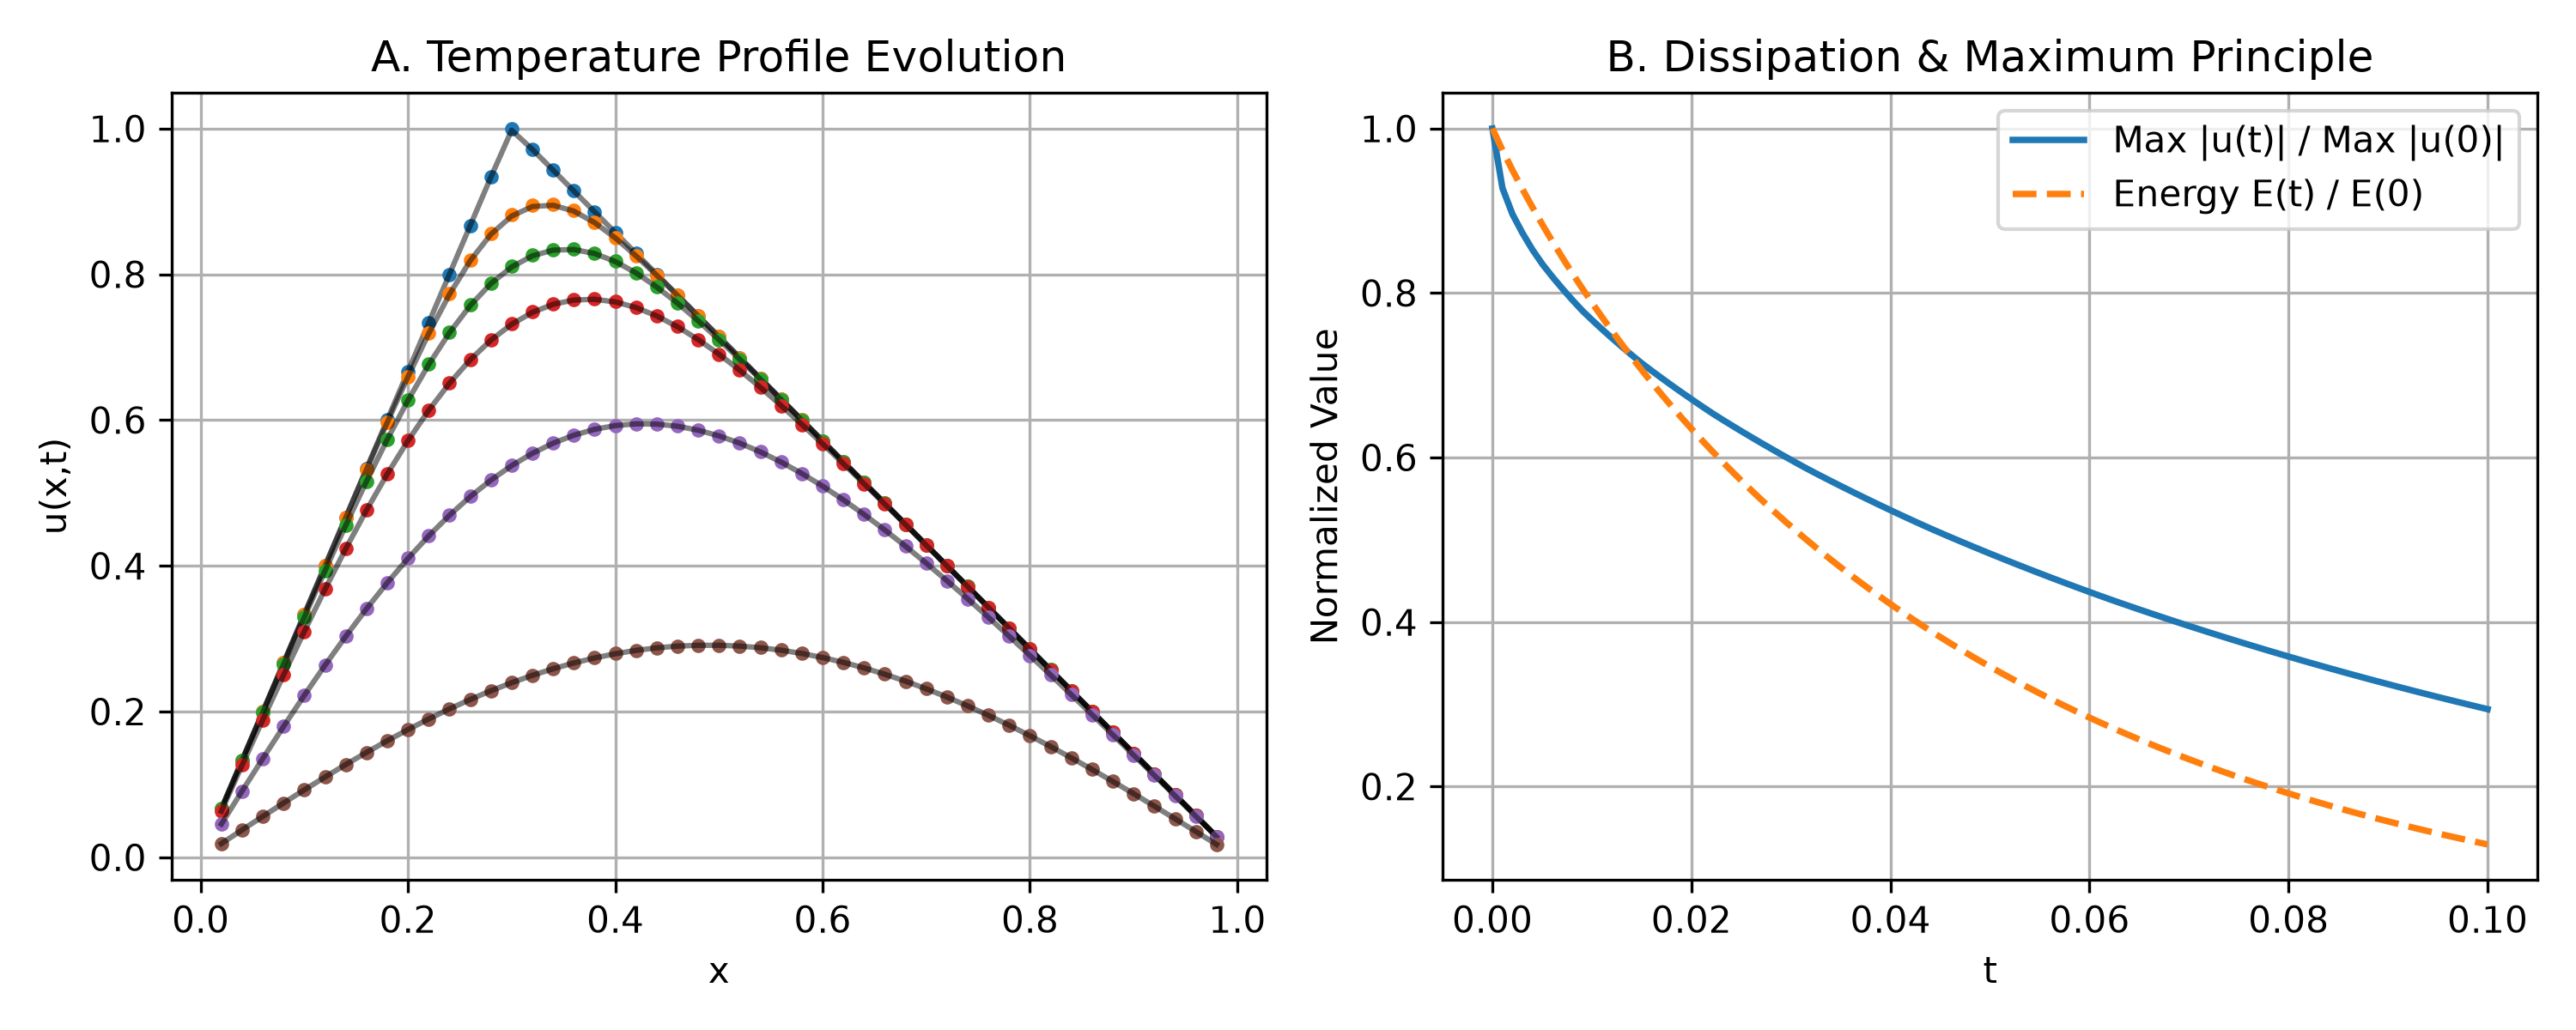
\includegraphics[width=\textwidth]{fig1_heat_decay.png}
\caption{Experiment H1. (A) RK4 points (dots) against the exact Fourier series (black lines) at
$t=0,0.002,0.005,0.01,0.03,0.1$. (B) Normalised maximum $\max_x u(t)/\max_x u(0)$ and normalised energy
$E(t)/E(0)$.}
\label{fig:heat1}
\end{figure}

\paragraph{Results.} Figure~\ref{fig:heat1}A shows that the RK4 points lie on the exact solution at
every time shown: the kink at $x=0.3$ is smoothed out immediately and the profile relaxes towards the
single hump of the first mode, with the high-frequency content dying first, as predicted by the rates
$\alpha(n\pi/L)^2$. Figure~\ref{fig:heat1}B shows that both the maximum and the energy decrease
monotonically, which confirms the maximum principle and the energy law $E'\le0$. The solution is a
faithful discrete heat flow.

\subsection{Experiment H2: spatial convergence}

\paragraph{Setup.} Hat profile, $T=0.1$, $N=19,39,79,159$, i.e.\ $h=0.05,0.025,0.0125,0.00625$ (the
kink at $x=0.3$ is then always a grid node). The RK4 step is $\Dt=0.2h^2$, so that the time error is
negligible, and the error is the maximum over the grid against the exact series.

\begin{table}[H]
\centering
\begin{tabular}{@{}cccc@{}}
\toprule
$N$ & $h$ & maximum error at $T=0.1$ & ratio\\
\midrule
19 & 0.05000 & $1.240\times10^{-3}$ & --\\
39 & 0.02500 & $3.095\times10^{-4}$ & 4.006\\
79 & 0.01250 & $7.737\times10^{-5}$ & 4.000\\
159 & 0.00625 & $1.934\times10^{-5}$ & 4.000\\
\bottomrule
\end{tabular}
\caption{Experiment H2: spatial convergence of the method-of-lines solution. The fitted slope in a
log--log plot is $2.00$.}
\label{tab:space}
\end{table}

\paragraph{Results.} Each halving of $h$ divides the error by $4.00$ (Table~\ref{tab:space},
Figure~\ref{fig:conv}A): the discretisation is second order in space, as the truncation term
$\tfrac{h^2}{12}u_{xxxx}$ predicts.

\subsection{Experiment H3: fourth-order convergence of RK4 and first order of Euler}

\paragraph{Design.} To expose the \emph{time} error one needs a reference without space error, i.e.\
the semi-discrete exact solution $e^{AT}\bfy_0$, and modes that are not yet dead, i.e.\ a short final time.
We therefore take the hat profile, $N=49$, $T=0.002$, and $n=16\cdot2^j$ steps ($j=0,\dots,5$), so that
$\Dt=T/n$ halves from row to row, from $1.25\times10^{-4}$ to $3.9\times10^{-6}$. These steps are
inside the stability limit of both methods.

\begin{table}[H]
\centering
\begin{tabular}{@{}rccc@{}}
\toprule
steps & $\Dt$ & Euler error & RK4 error\\
\midrule
16 & $1.25\times10^{-4}$ & $9.80\times10^{-4}$ & $7.40\times10^{-8}$\\
32 & $6.25\times10^{-5}$ & $4.89\times10^{-4}$ & $4.06\times10^{-9}$\\
64 & $3.13\times10^{-5}$ & $2.45\times10^{-4}$ & $2.39\times10^{-10}$\\
128 & $1.56\times10^{-5}$ & $1.22\times10^{-4}$ & $1.45\times10^{-11}$\\
256 & $7.81\times10^{-6}$ & $6.11\times10^{-5}$ & $8.88\times10^{-13}$\\
512 & $3.91\times10^{-6}$ & $3.06\times10^{-5}$ & $5.43\times10^{-14}$\\
\midrule
\multicolumn{2}{r}{fitted slope} & $1.00$ & $4.08$\\
\bottomrule
\end{tabular}
\caption{Experiment H3: maximum error at $T=0.002$ against the semi-discrete exact solution. The RK4
slope is fitted on the points above $10^{-13}$, since the last point is close to the round-off level.}
\label{tab:time}
\end{table}

\begin{figure}[H]
\centering
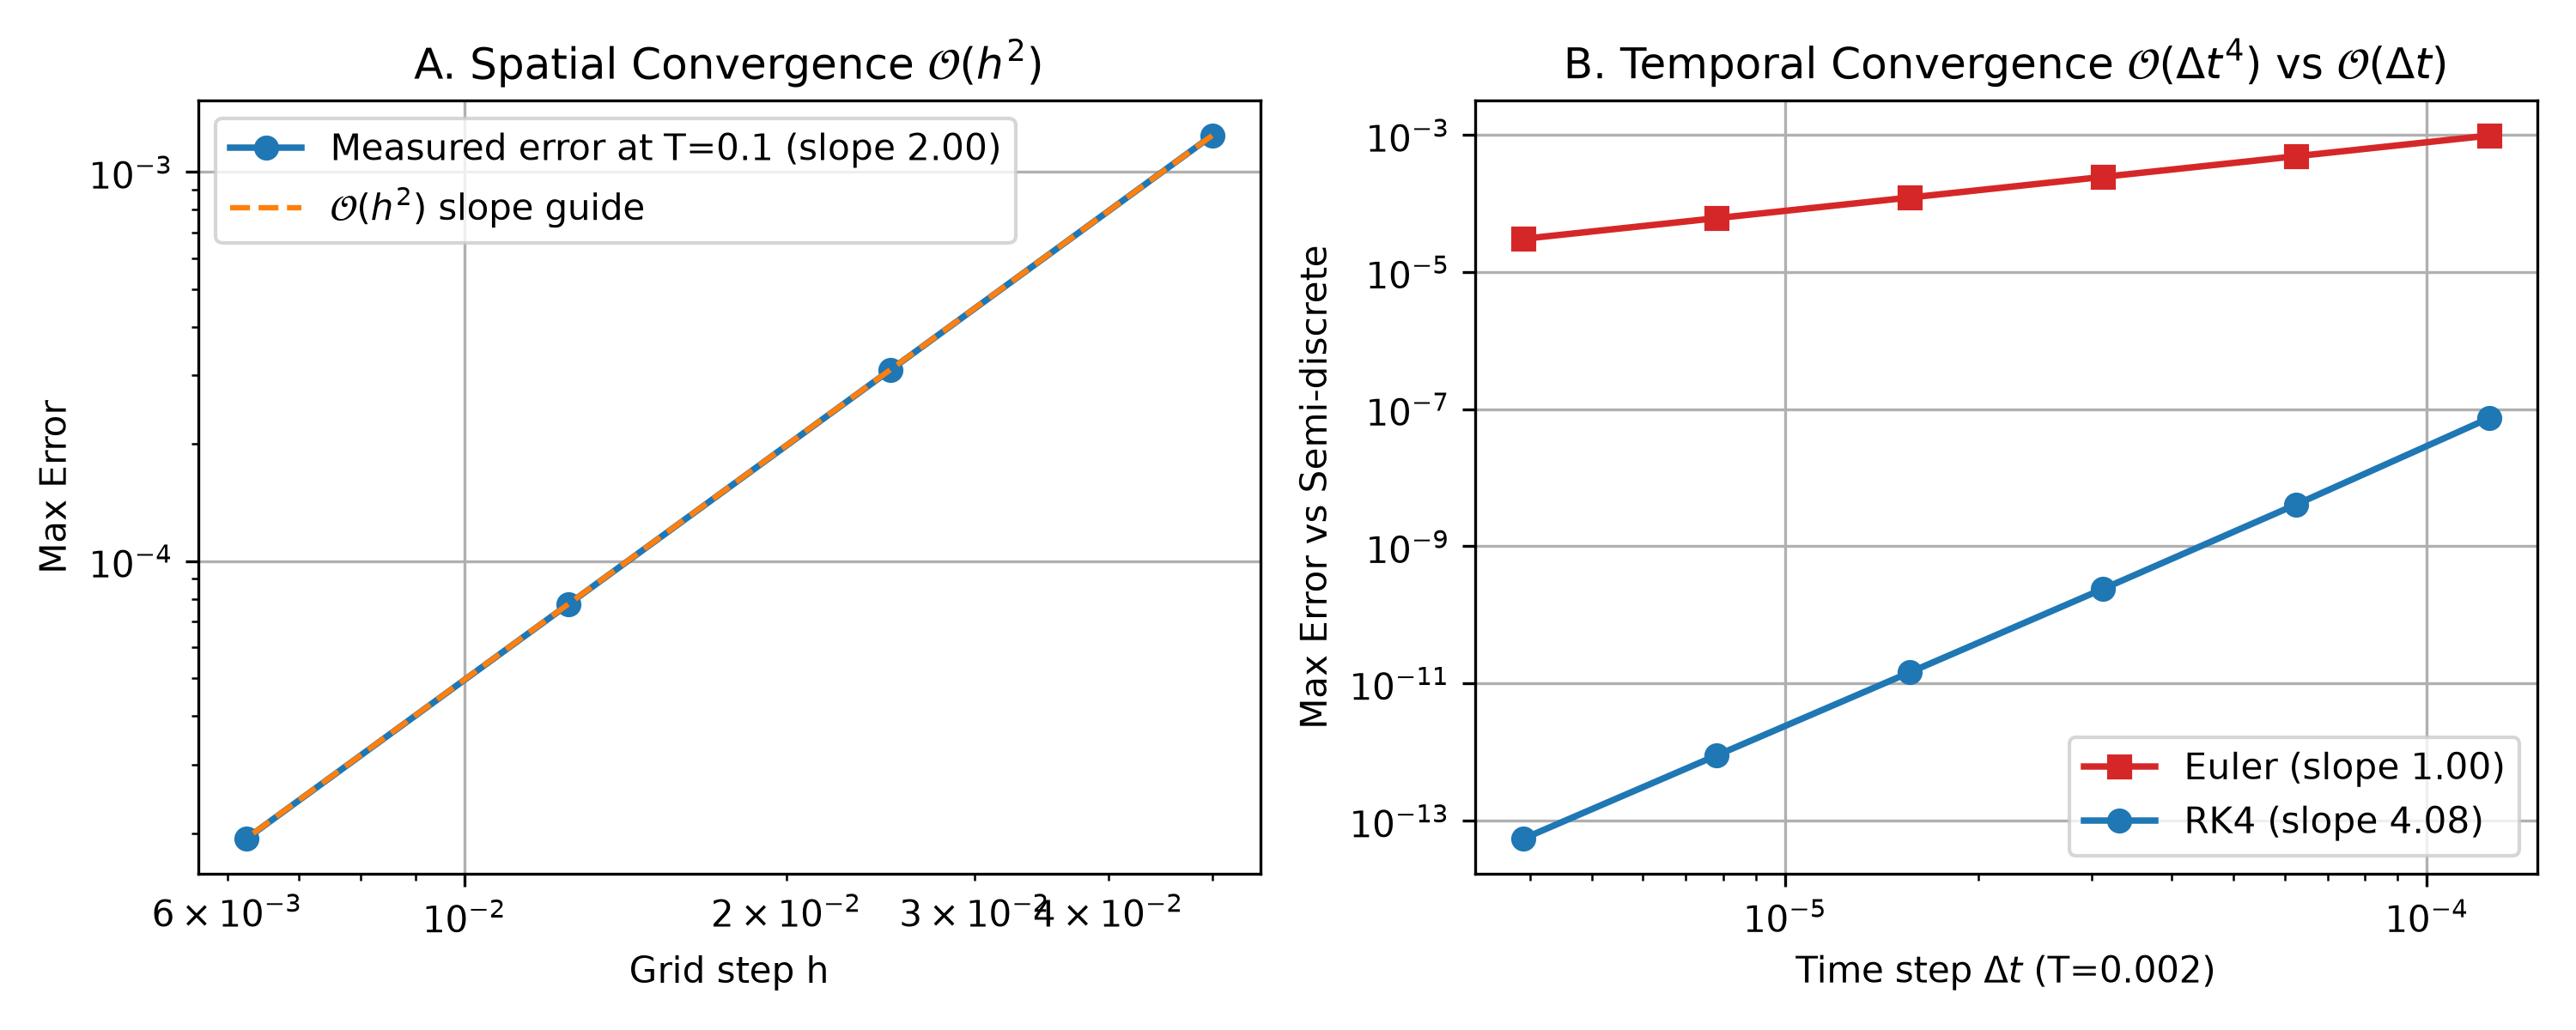
\includegraphics[width=\textwidth]{fig2_heat_convergence.png}
\caption{Experiments H2 and H3. (A) Spatial convergence: maximum error at $T=0.1$ against $h$, with an
$O(h^2)$ guide line. (B) Temporal convergence: Euler (slope 1) and RK4 (slope 4) against the
semi-discrete exact solution.}
\label{fig:conv}
\end{figure}

\paragraph{Results.} Halving $\Dt$ halves the Euler error (slope $1.00$) and divides the RK4 error by
about $16$ (slope $4.08$), which confirms the orders $1$ and $4$ derived in Section~\ref{sec:rk}
(Figure~\ref{fig:conv}B). The RK4 slope is slightly above $4$ because for the larger steps the neglected
higher terms $z^6,z^7,\dots$ of the exact factor $e^z$ still matter. The error of RK4 at the smallest
step is already near $5\times10^{-14}$: below roughly $10^{-13}$ double-precision round-off
($\approx2\times10^{-16}$ per operation, accumulated over many steps) would hide the fourth-order law,
so a convergence study should stop there. At equal step the RK4 error is smaller than that of Euler by
a factor of $10^{4}$ already at $\Dt=1.25\times10^{-4}$, at four times the cost per step.

\subsection{Experiment H4: the stability limit}

\paragraph{Setup.} Panel A of Figure~\ref{fig:heat3} plots $|R(z)|$ for Euler and RK4 on
$-4\le z\le0.5$. Panel B tests the limit~\eqref{eq:dtlimit} directly. The highest-frequency eigenmode
($\sin(N\pi x)$, with $\lambda_N=-9990.1$) is started with amplitude $10^{-15}$ and marched with RK4
for $250$ steps with $\Dt$ chosen so that $z=\lambda_N\Dt$ equals $0.95$ and $1.05$ times the RK4 limit
$z_{\mathrm{lim}}=-2.7853$.

\begin{figure}[H]
\centering
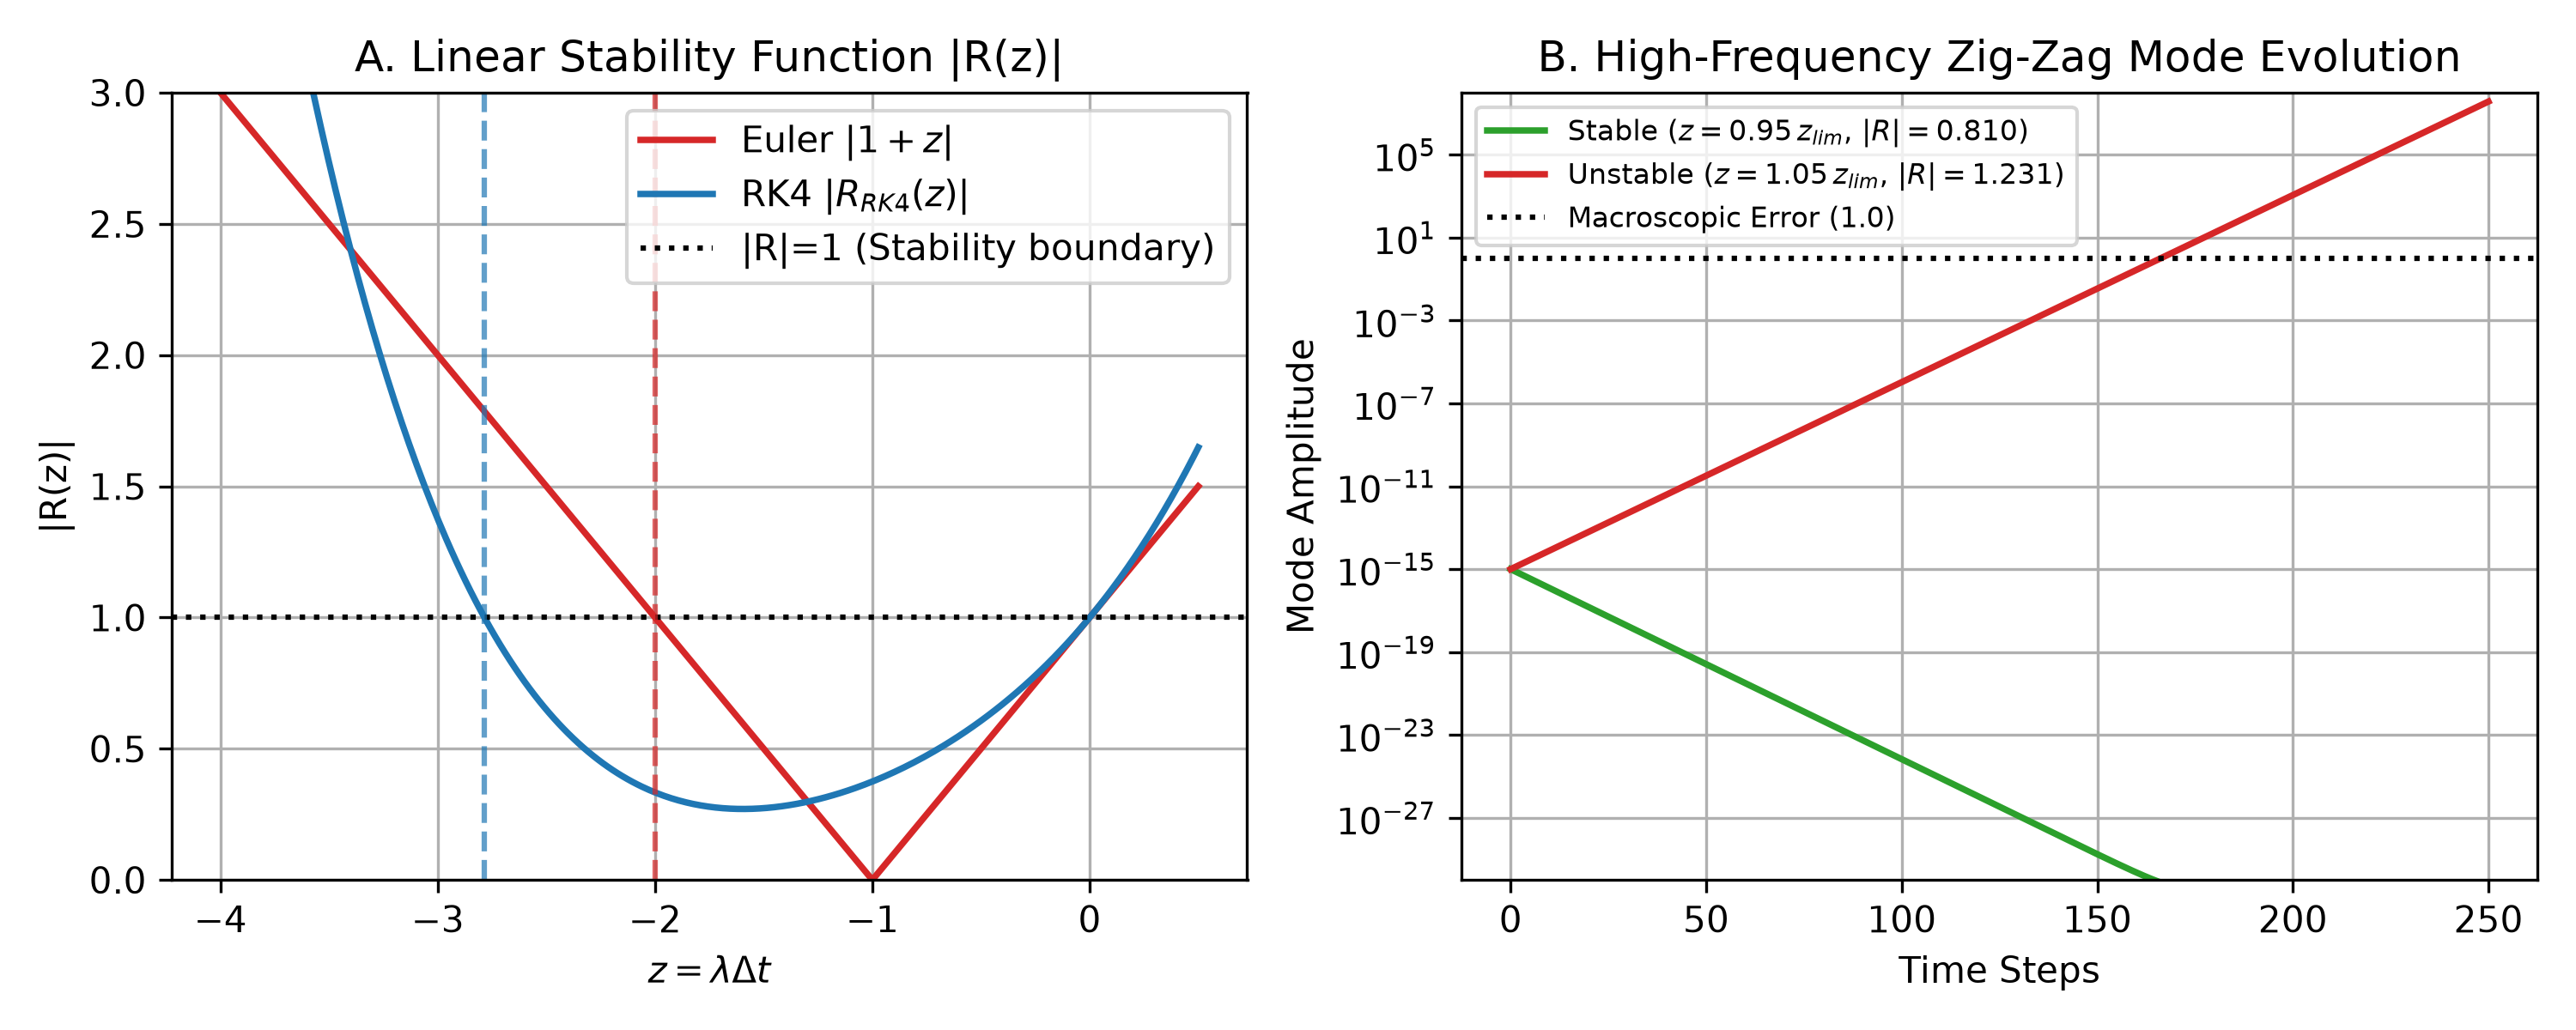
\includegraphics[width=\textwidth]{fig3_heat_stability.png}
\caption{Experiment H4. (A) Stability functions $|R(z)|$ of Euler and RK4; the dashed lines mark the
limits $z=-2$ and $z=-2.7853$. (B) Amplitude of the zig-zag mode started at $10^{-15}$ for
$z=0.95\,z_{\mathrm{lim}}$ (stable) and $z=1.05\,z_{\mathrm{lim}}$ (unstable).}
\label{fig:heat3}
\end{figure}

\paragraph{Results.} In panel A, $|R_{\mathrm{Euler}}|=|1+z|$ leaves the unit band at $z=-2$ and
$|R_{\mathrm{RK4}}|$ at $z=-2.7853$; the RK4 curve reaches its minimum $0.27$ near $z\approx-1.6$.
In panel B the mode inside the limit decays by a factor $|R|=0.810$ per step, whereas the mode only
$5\%$ beyond the limit grows by $|R|=1.231$ per step and, starting from round-off size $10^{-15}$,
reaches order one after about $170$ steps and then keeps growing. The measured growth of each curve matches the prediction
$|R(\lambda_N\Dt)|$, which confirms the stability function derived in Section~\ref{sec:stab}. The
blow-up is a purely numerical grid-scale zig-zag with no counterpart in the physics.

\subsection{What the heat experiments show}

On a linear, dissipative, exactly solvable problem RK4 behaves exactly as the theory says: fourth order
in time, with an $O(h^2)$ space error that dominates the total error; and a time step limited not by
accuracy but by stability, $\Dt\lesssim0.696\,h^2/\alpha$. Because the problem is linear, only the
four ``tall'' order conditions are tested (Section~\ref{sec:detect}, Table~\ref{tab:detect}), and
because it is dissipative errors decay instead of growing. The Lorenz system supplies the opposite
situation.

% ===============================================================
\section{The Lorenz System}\label{sec:lorenz}
% ===============================================================

\subsection{The equations}

The Lorenz system~\cite{lorenz1963} is the three-dimensional ODE
\begin{equation}
\dot x=\sigma(y-x),\qquad \dot y=x(\rho-z)-y,\qquad \dot z=xy-\beta z,
\label{eq:lorenz}
\end{equation}
obtained by Lorenz as a three-mode truncation of a model of thermal convection in a fluid layer heated
from below. The classical parameter values are $\sigma=10$, $\beta=8/3$, and $\rho$ is varied.
The system is of the form~\eqref{eq:ivp} with $\bfy=(x,y,z)$; it needs no spatial discretisation, so RK4
can be applied directly. The right-hand side is quadratic (the terms $xz$ and $xy$), hence nonlinear,
and no closed-form solution is known. It has the symmetry $(x,y,z)\mapsto(-x,-y,z)$.

\subsection{Equilibria and their stability}

Setting the right-hand side of~\eqref{eq:lorenz} to zero gives $y=x$, $\beta z=x^2$ and then
$x=0$ or $z=\rho-1$. The equilibria are the origin and, for $\rho>1$,
\begin{equation}
C_\pm=\Bigl(\pm\sqrt{\beta(\rho-1)},\ \pm\sqrt{\beta(\rho-1)},\ \rho-1\Bigr).
\end{equation}
Linearising about an equilibrium gives $\dot{\boldsymbol\delta}=J\boldsymbol\delta$ with
\begin{equation}
J(x,y,z)=\begin{pmatrix}-\sigma&\sigma&0\\ \rho-z&-1&-x\\ y&x&-\beta\end{pmatrix},
\end{equation}
which is the system $\bfy'=A\bfy$ of Section~\ref{sec:stab}: the equilibrium is stable if all
eigenvalues of $J$ have negative real part.

\paragraph{The origin.} The $z$-direction decouples with eigenvalue $-\beta<0$ and the remaining block
has characteristic polynomial $\lambda^2+(\sigma+1)\lambda+\sigma(1-\rho)=0$, whose constant term is
positive for $\rho<1$ (stable) and negative for $\rho>1$ (one positive root: unstable). For $\rho=28$,
$\lambda=(-11\pm\sqrt{1201})/2=11.83,\,-22.83$, together with $-8/3$: the origin is a saddle.

\paragraph{The convection states $C_\pm$.} Their characteristic polynomial is
\begin{equation}
\lambda^3+a\lambda^2+b\lambda+c=0,\qquad a=\sigma+\beta+1,\ \ b=\beta(\sigma+\rho),\ \ c=2\sigma\beta(\rho-1).
\end{equation}
All coefficients are positive for $\rho>1$. Stability can be lost only when a root crosses the imaginary
axis; a crossing at $\lambda=i\omega$ requires $c=ab$ (then $\omega^2=b$). Solving $c=ab$ for $\rho$ gives
the Hopf value
\begin{equation}
\rho_H=\frac{\sigma(\sigma+\beta+3)}{\sigma-\beta-1}=24.74\quad(\sigma=10,\ \beta=\tfrac83).
\end{equation}
For $1<\rho<\rho_H$ the points $C_\pm$ are stable (steady convection); for $\rho>\rho_H$ both are unstable
spirals and no stable equilibrium is left. At $\rho=28$ the eigenvalues at $C_\pm$ are one real root
$\approx-13.85$ and a complex pair $0.094\pm10.19\,i$. For $\rho$ slightly below $\rho_H$ (from about
$24.06$) it is known~\cite{sparrow1982} that a chaotic set coexists with the stable points $C_\pm$.

\begin{table}[H]
\centering
\begin{tabular}{@{}ll@{}}
\toprule
range of $\rho$ & behaviour\\
\midrule
$0<\rho<1$ & only the origin exists and it is stable: all motion decays to rest\\
$1<\rho<\rho_H\approx24.74$ & $C_\pm$ are stable: motion settles into steady convection\\
$\rho>\rho_H$ & no stable equilibrium; chaotic motion at $\rho=28$\\
\bottomrule
\end{tabular}
\caption{Route from rest to chaos in the Lorenz system for $\sigma=10$, $\beta=8/3$.}
\label{tab:route}
\end{table}

\subsection{Dissipation, boundedness and chaos}

The divergence of the right-hand side is constant,
\begin{equation}
\frac{\partial\dot x}{\partial x}+\frac{\partial\dot y}{\partial y}+\frac{\partial\dot z}{\partial z}
=-(\sigma+1+\beta)=-13.667,
\end{equation}
so a small blob of initial conditions has its volume multiplied by $e^{-13.667\,t}$, a factor of about
$10^{-6}$ after one time unit. Moreover all trajectories enter and stay in a bounded ellipsoid
(consider $V=x^2+y^2+(z-\sigma-\rho)^2$, for which $\dot V<0$ far from the origin). The long-time motion
therefore lives on a set of zero volume, but when all equilibria are unstable it neither settles at a
point nor on a simple loop: this is the \emph{strange attractor}.

Chaos means sensitive dependence on initial conditions: two nearby trajectories separate like
$|\delta(t)|\approx|\delta(0)|e^{\lambda_1t}$, where $\lambda_1$ is the largest \emph{Lyapunov exponent}.
The three exponents $\lambda_1\ge\lambda_2\ge\lambda_3$ can be computed by advancing the Lorenz
equations together with three perpendicular displacement vectors by the variational equation
$\dot{\boldsymbol\delta}=J(\bfy(t))\boldsymbol\delta$ and re-orthonormalising them by a QR
decomposition at regular intervals (Algorithm~\ref{alg:lyap}); $\lambda_i$ is the time average of
$\ln R_{ii}$. For $\sigma=10,\rho=28,\beta=8/3$ the values reported in the literature are
$\lambda_1\approx+0.906$, $\lambda_2=0$, $\lambda_3\approx-14.57$; their sum equals the divergence
$-13.667$ (the sum rule is a check for any implementation), and the pattern $(+,0,-)$ is the signature
of a chaotic attractor. An error $\varepsilon$ grows to the size of the attractor in a time of order
$\lambda_1^{-1}\ln(\Delta/\varepsilon)$, so long single trajectories cannot be reproduced; only
exponents, statistics and short-time accuracy can.

\begin{algorithm}[H]
\caption{Lyapunov exponents of the Lorenz system (Benettin's method)}\label{alg:lyap}
\begin{algorithmic}[1]
\State start on the attractor (discard a transient); $Q\gets I_3$; $S_i\gets0$ for $i=1,2,3$
\For{$m=1,\dots,N_{\mathrm{int}}$}
  \State advance $\bfy$ and the three columns of $Q$ over a short time $\tau$ with RK4
  \State \qquad (state: $\bfy'=\bff(\bfy)$; columns: $\delta'=J(\bfy)\delta$)
  \State $Q,R\gets \mathrm{QR}(\text{advanced columns})$
  \State $S_i\gets S_i+\ln|R_{ii}|$ for $i=1,2,3$
\EndFor
\State \Return $\lambda_i\gets S_i/(N_{\mathrm{int}}\,\tau)$
\end{algorithmic}
\end{algorithm}
% NOTE: the values above are the literature values. If you want to quote your own computed exponents from
% loretnz.py, add them here with the averaging time used.

\subsection{Choice of the time step}

The fastest decaying direction on the attractor is that of the origin, $\lambda=-22.83$, so RK4 is stable
for $\Dt\lesssim2.7853/22.83\approx0.12$ (Euler: $\Dt\lesssim0.088$). Contrary to the heat equation the
problem is therefore not stiff: it is \emph{accuracy}, not stability, that selects the step, and the
value $\Dt=0.01$ used below is well inside the stability limit.

% ===============================================================
\section{Lorenz System: Experiments}\label{sec:lorenzexp}
% ===============================================================

All runs use RK4 (Algorithm~\ref{alg:rk4}) with $\Dt=0.01$, $\sigma=10$, $\beta=8/3$ and the initial
point $(1,1,1)$.

\subsection{Experiment L1: the strange attractor at $\rho=28$}

The system is integrated for $4000$ steps ($t=40$) and the first $500$ steps are discarded as transient.

\begin{figure}[H]
\centering
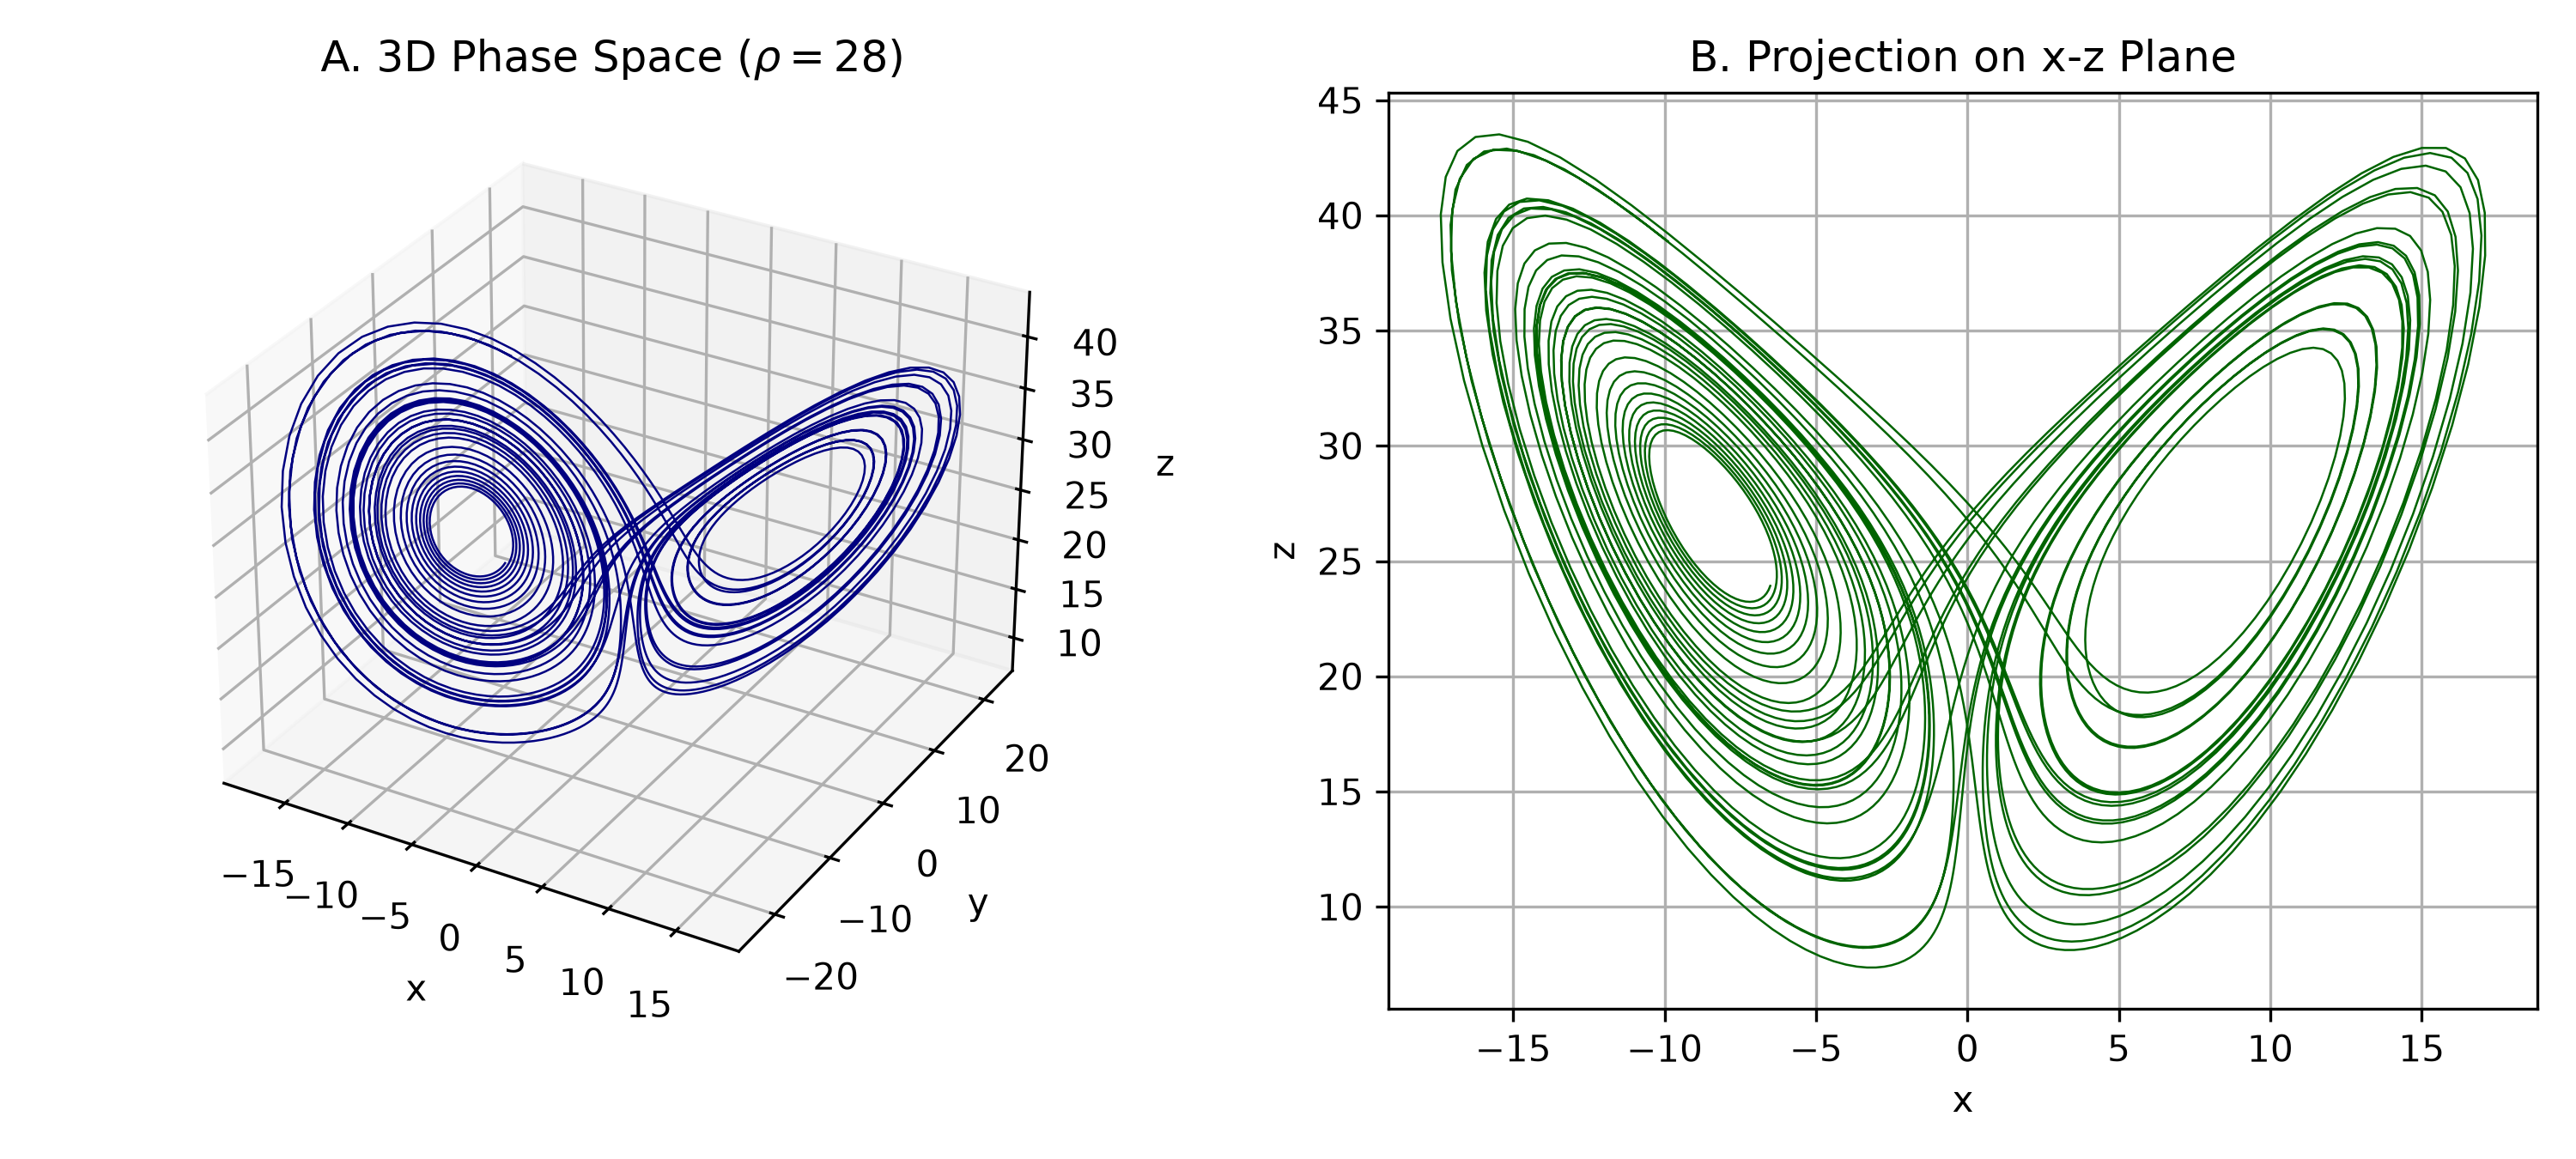
\includegraphics[width=\textwidth]{fig4_lorenz_attractor.png}
\caption{Experiment L1. Lorenz attractor for $\rho=28$: (A) three-dimensional phase space; (B) projection
on the $x$--$z$ plane.}
\label{fig:attractor}
\end{figure}

Figure~\ref{fig:attractor} shows the characteristic butterfly: the trajectory winds around the two
unstable convection points $C_\pm=(\pm8.485,\pm8.485,27)$, remains bounded, never closes on itself and
switches irregularly between the two wings. This is the numerical picture of the properties derived in
the previous section: no stable equilibrium (since $\rho>\rho_H$), boundedness, and a motion that is
neither steady nor periodic.

\subsection{Experiment L2: the route to chaos as $\rho$ changes}

Three values of $\rho$ are compared, in the $x$--$z$ plane, for the same initial point.
For $\rho=10$ and $\rho=24.5$ the run has $3000$ steps ($t=30$) with the first $300$ discarded;
for $\rho=100$ the transient is long, so $20000$ steps are used and the first $12000$ are discarded.

\begin{figure}[H]
\centering
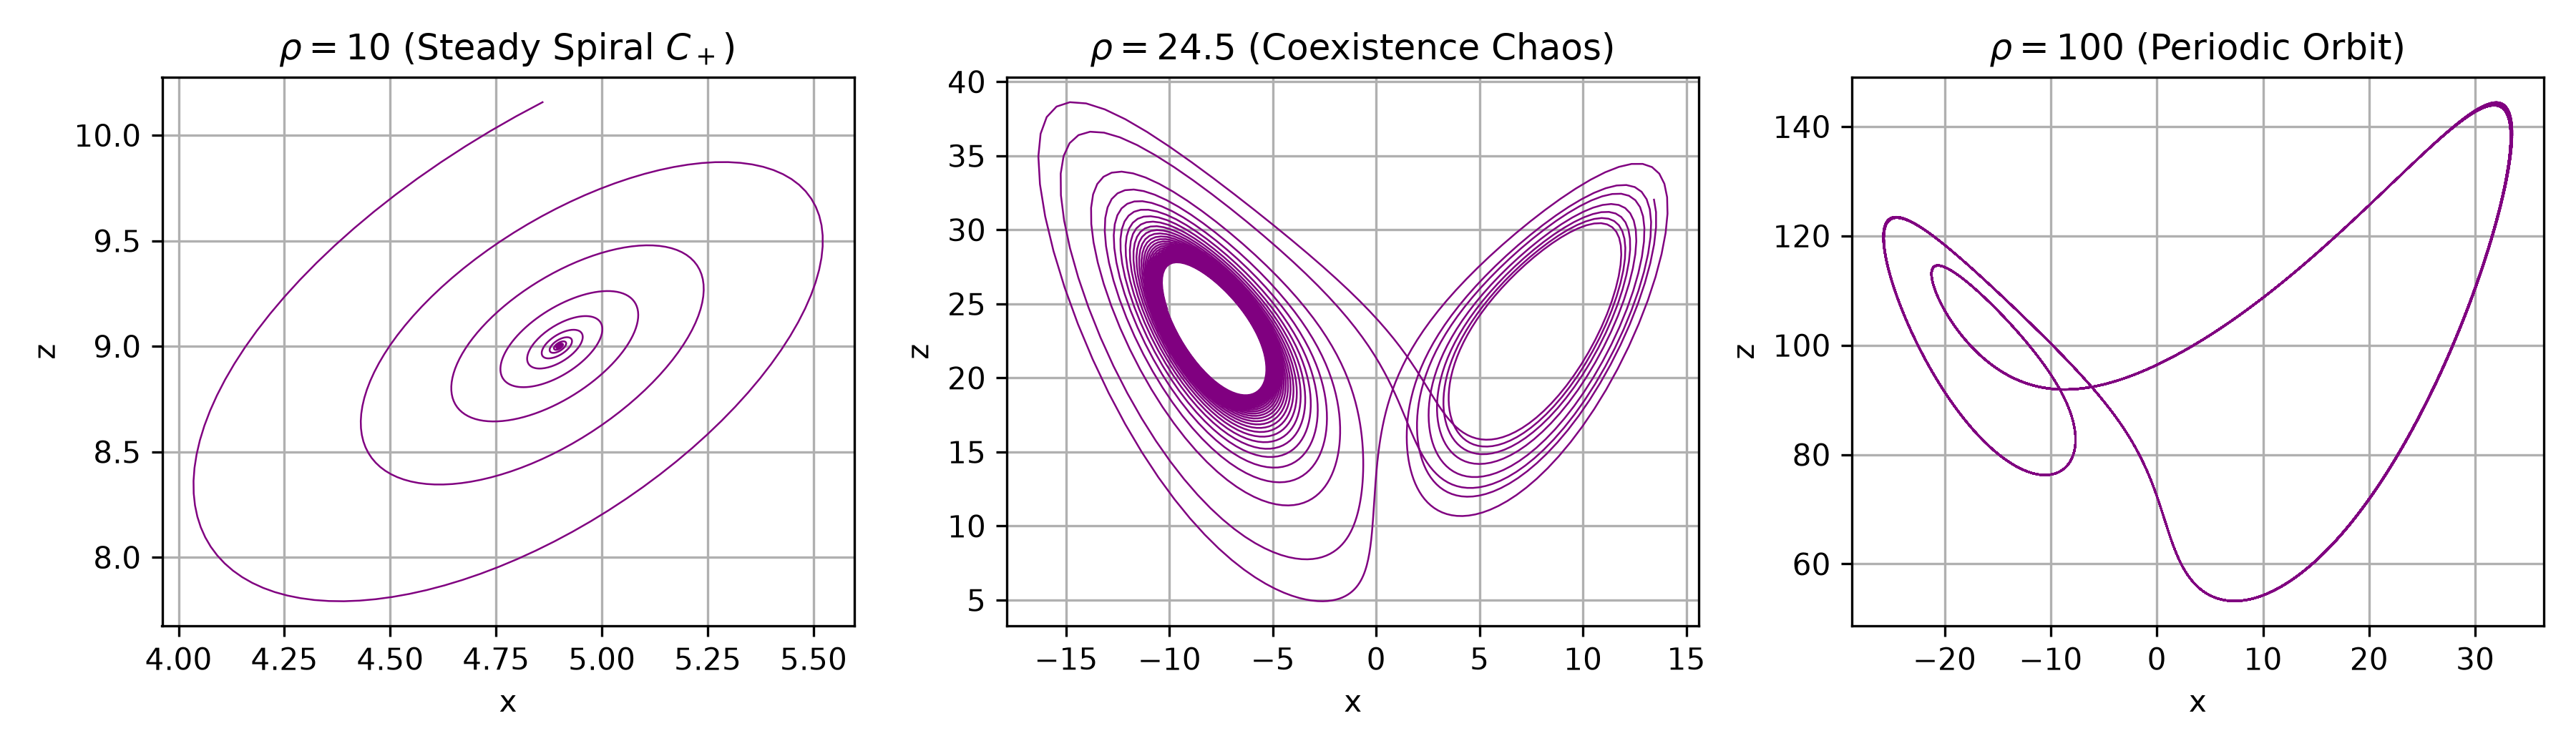
\includegraphics[width=\textwidth]{fig5_lorenz_bifurcation.png}
\caption{Experiment L2. Orbits in the $x$--$z$ plane: (left) $\rho=10$, a spiral into the stable
convection point $C_+$; (middle) $\rho=24.5$, below $\rho_H$ but inside the window where chaotic and
steady behaviour coexist; (right) $\rho=100$, a periodic orbit.}
\label{fig:rho}
\end{figure}

\begin{itemize}[leftmargin=*]
\item \textbf{$\rho=10$:} the orbit spirals into $C_+=(4.90,4.90,9)$ and stops there, as predicted for
$1<\rho<\rho_H$ (all eigenvalues of $J$ at $C_\pm$ have negative real part).
\item \textbf{$\rho=24.5$:} this value lies between $24.06$ and $\rho_H=24.74$, where the stable points
$C_\pm$ and a chaotic set coexist; the trajectory shown has a long irregular excursion around the wings
before the end of the run, with many turns around one convection point and only a few around the other.
The long-time fate of a single trajectory in this window depends on the initial point and cannot be read
off from a run of this length.
\item \textbf{$\rho=100$:} chaos is not monotone in $\rho$. For $\rho$ near $100$ the system has a
stable periodic orbit, and once the transient has been removed the trajectory retraces a closed loop.
\end{itemize}

% ===============================================================
\section{The Lid-Driven Cavity Problem}\label{sec:cavity}
% ===============================================================

This section applies the method of lines and RK4 to a two-dimensional nonlinear PDE problem. The
physics is not discussed beyond what is needed to write the equations.

\subsection{Governing equations and the streamfunction--vorticity form}

In the unit square $\Omega=[0,1]^2$ the incompressible Navier--Stokes equations for the velocity
$\mathbf u=(u,v)$ and pressure $p$ are
\begin{align}
\nabla\cdot\mathbf u&=0,\\
\mathbf u_t+(\mathbf u\cdot\nabla)\mathbf u&=-\nabla p+\frac1{Re}\,\Delta\mathbf u,
\end{align}
with $\mathbf u=(1,0)$ on the top side $y=1$ (the moving lid) and $\mathbf u=\mathbf 0$ on the other three
sides. As a time-dependent problem for $(u,v,p)$ this is a differential--algebraic system, because $p$
has no time derivative, so it cannot be fed directly to an RK method. The pressure is eliminated by the
\emph{streamfunction--vorticity formulation}:
\begin{equation}
u=\frac{\partial\psi}{\partial y},\quad v=-\frac{\partial\psi}{\partial x},\qquad
\omega=\frac{\partial v}{\partial x}-\frac{\partial u}{\partial y}=-\Delta\psi .
\end{equation}
The first definition satisfies $\nabla\cdot\mathbf u=0$ identically. Taking the curl of the momentum
equation removes $p$ and leaves two equations:
\begin{align}
\frac{\partial\omega}{\partial t}&=-\Bigl(u\frac{\partial\omega}{\partial x}+v\frac{\partial\omega}{\partial y}\Bigr)
+\frac1{Re}\Bigl(\frac{\partial^2\omega}{\partial x^2}+\frac{\partial^2\omega}{\partial y^2}\Bigr)
&&\text{(evolution equation)},\label{eq:vort}\\
\Delta\psi&=-\omega &&\text{(Poisson constraint)}.\label{eq:poisson}
\end{align}
The vorticity equation~\eqref{eq:vort} is a nonlinear advection--diffusion PDE with one time derivative,
so it is the one to which the method of lines is applied. At every instant the velocity field needed on
its right-hand side is obtained from $\omega$ through the Poisson equation~\eqref{eq:poisson}.

\subsection{Boundary conditions}

On all walls $\psi=0$ (no flow through the wall). The condition that fixes the vorticity on the wall
follows from a Taylor expansion of $\psi$ (Thom's formula~\cite{thom1933}). On a wall with tangential velocity
$U_{\mathrm{wall}}$ and $\psi_{\mathrm{wall}}=0$, with $\psi_1$ the value one grid step $h_s$ inside,
\begin{equation}
\omega_{\mathrm{wall}}=-\frac{2\psi_1}{h_s^2}-\frac{2U_{\mathrm{wall}}}{h_s}\quad(\text{moving lid}),\qquad
\omega_{\mathrm{wall}}=-\frac{2\psi_1}{h_s^2}\quad(\text{fixed walls}).
\end{equation}
For the lid, $U_{\mathrm{wall}}=1$; the sign is that of $\omega=-\partial u/\partial y$ at the lid.

\subsection{Method of lines}

Divide the square into a uniform grid with $N_c=41$ points in each direction, $h_s=1/(N_c-1)=0.025$,
and let $\omega_{i,j}(t)\approx\omega(x_i,y_j,t)$, $\psi_{i,j}(t)\approx\psi(x_i,y_j,t)$. Central
differences replace all space derivatives:
\begin{align}
(\Delta\omega)_{i,j}&\approx\frac{\omega_{i+1,j}+\omega_{i-1,j}+\omega_{i,j+1}+\omega_{i,j-1}-4\omega_{i,j}}{h_s^2},\\
\Bigl(\frac{\partial\omega}{\partial x}\Bigr)_{i,j}&\approx\frac{\omega_{i+1,j}-\omega_{i-1,j}}{2h_s},\quad
\Bigl(\frac{\partial\omega}{\partial y}\Bigr)_{i,j}\approx\frac{\omega_{i,j+1}-\omega_{i,j-1}}{2h_s},\\
u_{i,j}&\approx\frac{\psi_{i,j+1}-\psi_{i,j-1}}{2h_s},\quad
v_{i,j}\approx-\frac{\psi_{i+1,j}-\psi_{i-1,j}}{2h_s}.
\end{align}
Collecting the vorticity at all interior nodes into one vector $\bfy(t)\in\R^{M}$, $M=(N_c-2)^2=1521$,
the evolution equation becomes
\begin{equation}
\frac{\dd\omega_{i,j}}{\dd t}=-\Bigl(u_{i,j}\frac{\omega_{i+1,j}-\omega_{i-1,j}}{2h_s}
+v_{i,j}\frac{\omega_{i,j+1}-\omega_{i,j-1}}{2h_s}\Bigr)
+\frac{1}{Re\,h_s^2}\bigl(\omega_{i+1,j}+\omega_{i-1,j}+\omega_{i,j+1}+\omega_{i,j-1}-4\omega_{i,j}\bigr),
\end{equation}
that is, $\bfy'=\bff(\bfy)$ in the form~\eqref{eq:ivp}, with $\bff$ nonlinear. The streamfunction
needed in $u,v$ is the solution of the discrete Poisson problem. In matrix form, with the
one-dimensional second-difference matrix $D=\mathrm{tridiag}(1,-2,1)\in\R^{m\times m}$, $m=N_c-2$, the
five-point Laplacian on the interior is the Kronecker sum
\begin{equation}
L_h=\frac1{h_s^2}\bigl(I_m\otimes D+D\otimes I_m\bigr),\qquad L_h\,\boldsymbol\psi=-\mathbf y .
\end{equation}
The matrix $L_h$ is sparse and constant in time, so it is factorised once (sparse LU) and the
factorisation is reused in every step.

\subsection{Time integration with RK4}

The initial state is the fluid at rest, $\omega=\psi=0$. Each step of the computation is: (i) compute
the wall vorticity from the current $\psi$; (ii) advance the interior vorticity by one RK4 step
(Algorithm~\ref{alg:cavity}); (iii) solve the Poisson equation for the new $\psi$.

\begin{algorithm}[H]
\caption{Lid-driven cavity: method of lines with RK4}\label{alg:cavity}
\begin{algorithmic}[1]
\State set $\omega\gets0$, $\psi\gets0$; factorise $L_h$ once
\For{$n=1,2,\dots$ until steady state}
  \State $\omega_{\mathrm{wall}}\gets$ Thom's formula from $\psi$ \Comment{boundary values}
  \State $\bfy\gets\omega_{\mathrm{interior}}$; $u,v\gets$ central differences of $\psi$
  \State $k_1\gets\bff(\bfy)$; $\ k_2\gets\bff(\bfy+\tfrac12\Dt k_1)$; $\ k_3\gets\bff(\bfy+\tfrac12\Dt k_2)$; $\ k_4\gets\bff(\bfy+\Dt k_3)$
  \State $\bfy\gets\bfy+\tfrac{\Dt}{6}(k_1+2k_2+2k_3+k_4)$
  \State solve $L_h\boldsymbol\psi=-\bfy$ \Comment{new streamfunction, reusing the LU factors}
  \If{$\max|\bfy_{\mathrm{new}}-\bfy_{\mathrm{old}}|/\Dt<10^{-7}$} \State \textbf{stop} \EndIf
\EndFor
\end{algorithmic}
\end{algorithm}

\begin{remark}
In Algorithm~\ref{alg:cavity} the streamfunction (and so the velocity field and the wall vorticity)
is held fixed during the four RK4 stages and updated only after the step. The scheme therefore does
\emph{not} have fourth-order accuracy in time for the coupled problem; the RK4 structure gives good
stability and accuracy for the vorticity transport itself, and is used here to march to the steady
state, for which the temporal accuracy of the transient does not matter. A fully fourth-order treatment
would solve the Poisson equation inside every stage.
\end{remark}

\paragraph{Parameters and stability.} $Re=100$, $N_c=41$ ($h_s=0.025$), $\Dt=0.005$. The fastest
diffusive eigenvalue is about $-8/(Re\,h_s^2)=-128$, so $|\lambda|\Dt=0.64$, well inside the RK4 limit
$2.7853$; the advective limit $\approx2.83\,h_s/(2U)\approx0.035$ is also satisfied. The explicit
stability limit for the diffusive part scales as $\Dt\lesssim0.35\,Re\,h_s^2$, i.e.\ it shrinks
quadratically with the grid spacing: this is the same stiffness as in the heat equation, and the reason
why implicit or diagonally implicit RK methods (Section~\ref{sec:stab}) become attractive on fine grids.
The iteration is stopped when $\max|\Delta\omega|/\Dt<10^{-7}$.

\subsection{Results}

The run reaches the stopping criterion after $6172$ steps, i.e.\ at $t\approx30.9$. It is important that
the time interval is long enough: with a short time interval (of order $t\approx1$) the lid has only
influenced a thin layer under it, the interior velocity is nearly zero and no vortex has yet formed;
about $20$--$30$ time units are needed at $Re=100$ for the flow to reach its steady state.

\begin{figure}[H]
\centering
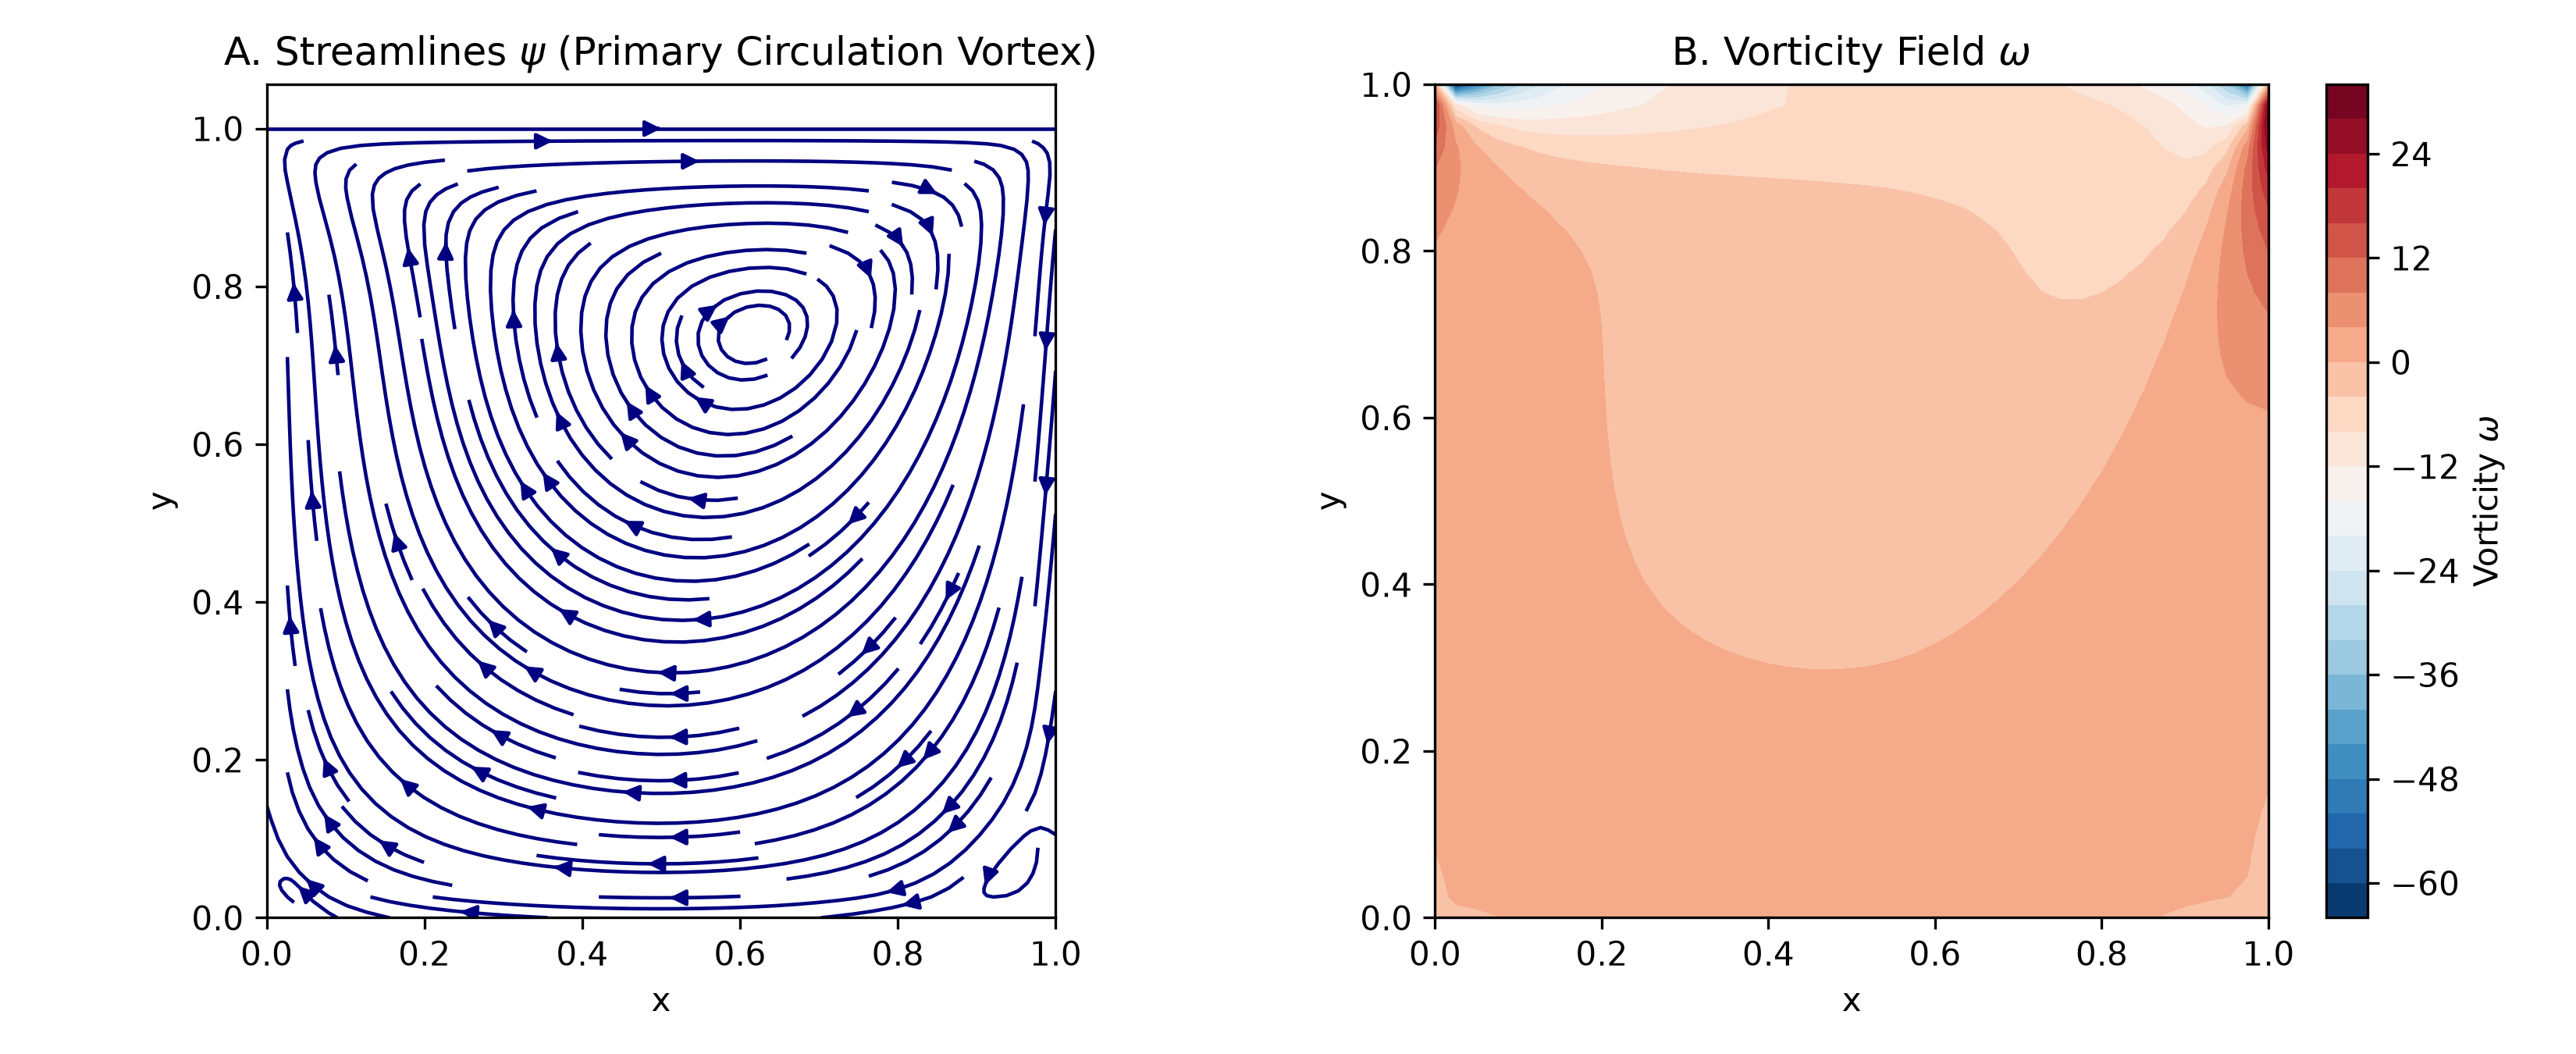
\includegraphics[width=\textwidth]{fig6_cavity_streamlines_vorticity.png}
\caption{Lid-driven cavity at $Re=100$ (steady state, $41\times41$ grid, RK4). (A) Streamlines. (B)
Vorticity field.}
\label{fig:cavity}
\end{figure}

Figure~\ref{fig:cavity}A shows one large primary vortex whose centre lies in the upper half of the
cavity, to the right of the middle, together with small counter-rotating eddies in the two lower
corners. Figure~\ref{fig:cavity}B shows strong negative vorticity along the lid, where the shear is
injected, with the largest gradients at the two upper corners (where the lid meets the fixed walls and
the boundary conditions are discontinuous), and nearly uniform weak vorticity in the interior.

\paragraph{Validation against a benchmark.} The classical benchmark for this problem is the table of
Ghia, Ghia and Shin~\cite{ghia1982} for $Re=100$. Figure~\ref{fig:ghia} compares the horizontal velocity
$u(0.5,y)$ along the vertical centre line and the vertical velocity $v(x,0.5)$ along the horizontal
centre line with their values.

\begin{figure}[H]
\centering
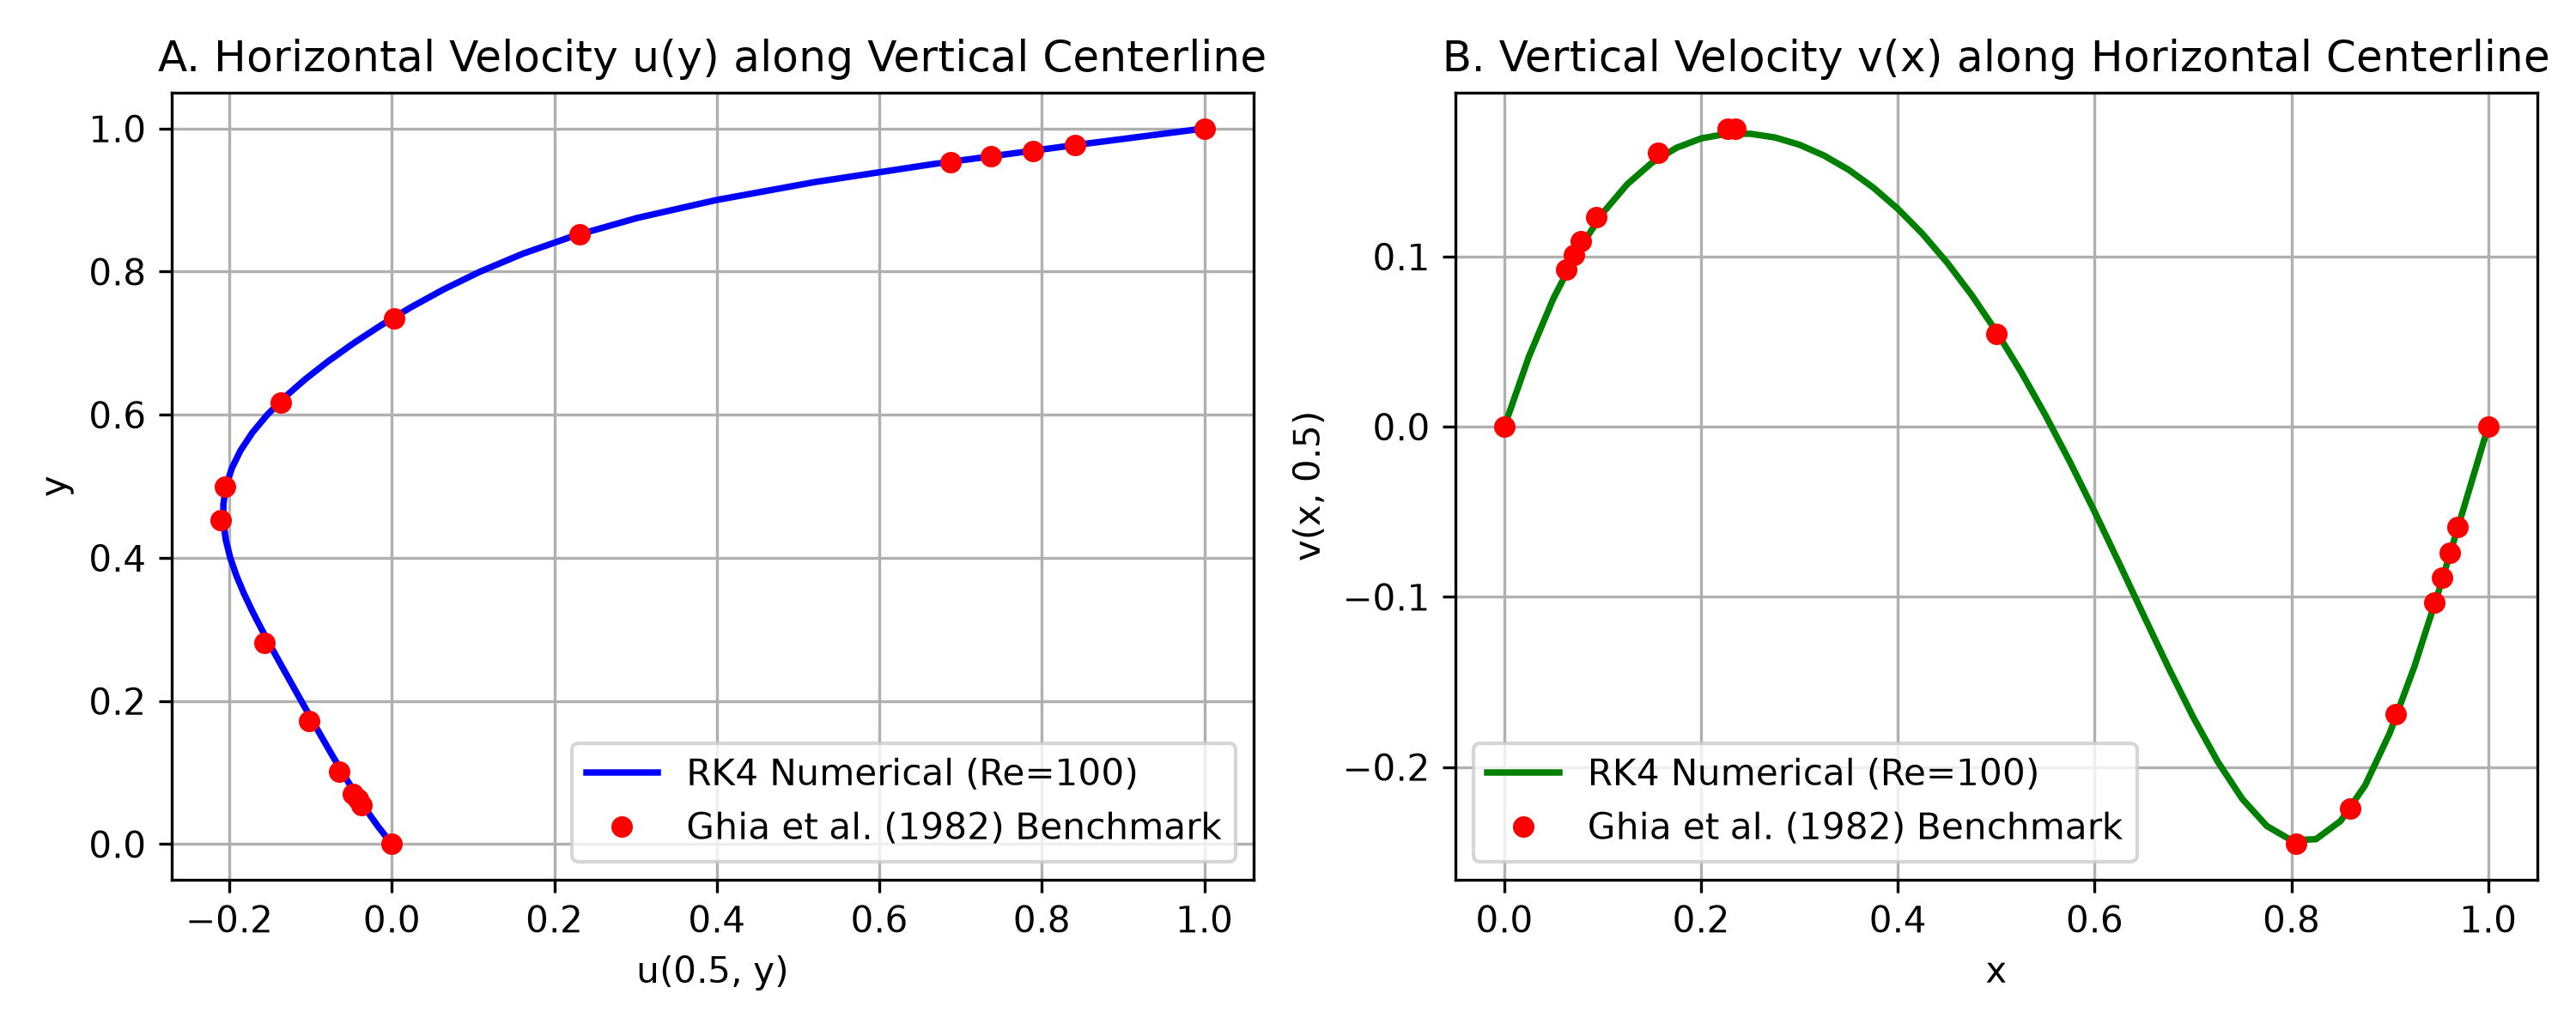
\includegraphics[width=\textwidth]{fig7_cavity_re_profiles.png}
\caption{Centre-line velocity profiles at $Re=100$ against the benchmark data of Ghia et
al.~\cite{ghia1982} (dots). (A) $u(0.5,y)$. (B) $v(x,0.5)$.}
\label{fig:ghia}
\end{figure}

The numerical curves pass through the benchmark points. Interpolating the computed profiles linearly
to the benchmark stations, the largest absolute difference is $0.0053$ for $u$ and $0.0034$ for $v$
(relative to the lid speed $1$), which is of the size expected from a $41\times41$ second-order grid.
The computed vertical velocity ranges between about $-0.25$ and $+0.18$, as in the benchmark.

% ===============================================================
\section{Discussion and Conclusions}
% ===============================================================

\paragraph{Theory.} An RK method is described by its Butcher tableau; comparing the Taylor series of the
exact and numerical solutions tree by tree shows that its order is decided by the identities
$\Phi(\vartheta)=1/\gamma(\vartheta)$ (Theorem~\ref{thm:order}). RK4 satisfies the eight conditions up to order four
(Table~\ref{tab:orderconds}) and fails all nine conditions of order five (Table~\ref{tab:order5}), so its order is exactly
four and its local error is $O(\Dt^5)$, while Euler satisfies only the first condition. Explicit methods need at least
$s=p$ stages and $s>p$ for $p\ge5$, so four stages for order four is the best possible ratio. For $y'=\lambda y$ one step multiplies $y$ by a stability function; for RK4 this
is the degree-four Taylor polynomial of $e^z$, which limits $|\lambda|\Dt$ to $2.7853$ against $2$ for Euler.

\paragraph{Heat equation.} The method of lines turns the heat equation into the linear system
$\bfy'=A\bfy$, which is stiff ($|\lambda|_{\max}\approx4\alpha/h^2$). The experiments confirm temporal
order $4.08$ for RK4 and $1.00$ for Euler, spatial order $2.00$, a monotone decay of energy and maximum,
and a sharp stability threshold: $0.95$ and $1.05$ times the limit give per-step factors $0.810$ and
$1.231$. The total error is dominated by the $O(h^2)$ space error, and the time step is chosen by
stability, not accuracy.

\paragraph{Lorenz system.} A nonlinear, non-stiff, chaotic ODE system is integrated directly by RK4. The
experiments show the strange attractor at $\rho=28$, a steady spiral at $\rho=10$ and a periodic orbit
at $\rho=100$, in agreement with the equilibrium and Hopf analysis; here the step is limited by accuracy
($\Dt=0.01$ against a stability limit $\approx0.12$), and sensitive dependence on initial conditions means
that only short-time accuracy, exponents and statistics are meaningful.

\paragraph{Lid-driven cavity.} A nonlinear PDE problem is reduced by the streamfunction--vorticity
formulation and the method of lines to an ODE system for $1521$ vorticity values, coupled with a Poisson
solve for the streamfunction, and marched with RK4 to steady state. The centre-line velocities agree with
the benchmark of Ghia et al.\ to within $0.006$. The explicit scheme is restricted by
$\Dt\lesssim0.35\,Re\,h_s^2$, which motivates implicit and diagonally implicit RK methods on finer grids.

\paragraph{Limitations.} The implicit methods (DIRK, Newton iteration) are described theoretically but
were not implemented; the cavity scheme holds $\psi$ fixed within a step and is not fourth-order in time;
the spatial discretisation is second order, so on all PDE problems the total accuracy is limited by
space and not by RK4.

% ===============================================================
\section*{Reproducibility}
% ===============================================================
All figures of this report are generated by one Python script, \texttt{experiment.py}, using NumPy,
SciPy and Matplotlib. The correspondence is: \texttt{fig1\_heat\_decay.png} (Figure~\ref{fig:heat1}),
\texttt{fig2\_heat\_convergence.png} (Figure~\ref{fig:conv}), \texttt{fig3\_heat\_stability.png}
(Figure~\ref{fig:heat3}), \texttt{fig4\_lorenz\_attractor.png} (Figure~\ref{fig:attractor}),
\texttt{fig5\_lorenz\_bifurcation.png} (Figure~\ref{fig:rho}),
\texttt{fig6\_cavity\_streamlines\_vorticity.png} (Figure~\ref{fig:cavity}) and
\texttt{fig7\_cavity\_re\_profiles.png} (Figure~\ref{fig:ghia}).

% ===============================================================
\begin{thebibliography}{9}
\bibitem{butcher2008} J.~C.~Butcher, \emph{Numerical Methods for Ordinary Differential Equations},
2nd ed., Wiley, 2008.
\bibitem{hairer1993} E.~Hairer, S.~P.~N{\o}rsett and G.~Wanner, \emph{Solving Ordinary Differential
Equations I: Nonstiff Problems}, 2nd ed., Springer, 1993.
\bibitem{lorenz1963} E.~N.~Lorenz, Deterministic nonperiodic flow, \emph{J.\ Atmos.\ Sci.}\ \textbf{20}
(1963), 130--141.
\bibitem{sparrow1982} C.~Sparrow, \emph{The Lorenz Equations: Bifurcations, Chaos, and Strange
Attractors}, Springer, 1982.
\bibitem{ghia1982} U.~Ghia, K.~N.~Ghia and C.~T.~Shin, High-Re solutions for incompressible flow using
the Navier--Stokes equations and a multigrid method, \emph{J.\ Comput.\ Phys.}\ \textbf{48} (1982),
387--411.
\bibitem{thom1933} A.~Thom, The flow past circular cylinders at low speeds, \emph{Proc.\ R.\ Soc.\
Lond.\ A} \textbf{141} (1933), 651--669.
\bibitem{ghorai} S.~Ghorai, UGP reading material on Runge--Kutta methods (supervisor's notes).
\end{thebibliography}

\end{document}
